% Compile from the project root with:
% pdflatex -output-directory=reports reports/project_report.tex

\documentclass[11pt,a4paper]{article}

\usepackage[utf8]{inputenc}
\usepackage[T1]{fontenc}
\usepackage[english]{babel}
\usepackage{lmodern}
\usepackage{microtype}
\usepackage{geometry}
\usepackage{graphicx}
\usepackage{booktabs}
\usepackage{array}
\usepackage{tabularx}
\usepackage{amsmath}
\usepackage{amssymb}
\usepackage{float}
\usepackage{xcolor}
\usepackage[hidelinks]{hyperref}
\usepackage{caption}
\usepackage{subcaption}
\usepackage{enumitem}

\geometry{margin=2.5cm}
\setlength{\parskip}{0.6em}
\setlength{\parindent}{0pt}
\setlist[itemize]{leftmargin=1.2cm}
\setlist[enumerate]{leftmargin=1.2cm}

\graphicspath{
  {results/figures/}
  {results/roc_curves/}
  {results/score_distributions/}
  {results/tsne_umap/}
  {results/confusion_matrices/}
  {../results/figures/}
  {../results/roc_curves/}
  {../results/score_distributions/}
  {../results/tsne_umap/}
  {../results/confusion_matrices/}
}

\title{\textbf{Partial Replication of the STOOD-X Paper for Out-of-Distribution Detection in Computer Vision}\\[0.4em]
\large Comparative Study of Out-of-Distribution Detection Methods in Computer Vision with Statistical Evaluation using STOOD-X}
\author{
Leonel Silima\\
Luis Lucas\\[0.4em]
Computer Vision -- PDEEC\\
FEUP -- University of Porto
}
\date{Academic Year 2025/2026}

\begin{document}

\maketitle

\begin{abstract}
This project presents a partial and adapted replication of the STOOD-X paper, applied to the problem of Out-of-Distribution (OOD) detection in computer vision.
The objective was to reproduce, at a reduced scale, the central idea of the original paper: using internal neural network representations and feature-space distances to distinguish In-Distribution (ID) and OOD samples, while comparing this behavior with classical OOD detection methods.
A ResNet-18 model was trained on CIFAR-10, used as the known distribution, and evaluated against three OOD datasets: CIFAR-100, SVHN and MNIST.
The compared methods were Maximum Softmax Probability (MSP), Energy-based OOD Detection, ODIN, Mahalanobis distance, KNN and a simplified STOOD-X implementation.
The evaluation uses standard OOD metrics: AUROC, AUPR-IN, AUPR-OUT and FPR95.
The project also generates visualizations to support the experimental analysis, including ROC curves, score distributions, heatmaps, boxplots, t-SNE/UMAP projections and a confusion matrix.
Since this replication does not implement the complete original methodology, the report explicitly distinguishes between the components that were replicated and the simplifications that were introduced.
The results show that Energy and ODIN perform best on CIFAR-100 and MNIST, while KNN and the simplified STOOD-X approach perform best on SVHN.
\end{abstract}

\textbf{Keywords:} OOD detection; computer vision; CIFAR-10; ResNet-18; STOOD-X; KNN; ODIN; Energy Score.

\textbf{Repository:} \href{https://github.com/Silima1/OOD_DETECTION_CV_PROJECT}{https://github.com/Silima1/OOD\_DETECTION\_CV\_PROJECT}.

\section{Introduction}

Modern image classification models are usually trained under the assumption that test data come from the same distribution as the training data.
In practice, this assumption is often violated.
A classifier trained on CIFAR-10 may receive handwritten digits, street-view house numbers, textures or other objects that do not belong to any of the known classes.
Even so, a neural network will still produce a prediction and often assign high confidence to it.

Out-of-Distribution detection addresses this problem.
The goal is not only to classify an image, but also to estimate whether that image belongs to the distribution on which the model was trained.
This capability is important in critical systems, where a confident decision on an unknown input can be dangerous.

In this project, the problem is studied in a controlled setting as a partial replication of the STOOD-X paper by Sevillano-Garcia, Luengo and Herrera~\cite{stoodx2025}.
The model is trained on CIFAR-10, and several OOD detection methods are compared using CIFAR-100, SVHN and MNIST as out-of-distribution datasets.
The replication mainly focuses on the OOD detection component based on feature-space analysis.
The visual explainability component proposed in the original paper is not reproduced in this work.

\section{Framing as a Replication of the STOOD-X Paper}

The original STOOD-X paper proposes a methodology for OOD detection with two main parts.
The first part, STOOD, uses distances in the feature space and a nonparametric statistical test to decide whether a sample belongs to the known distribution.
The second part, X, adds concept-based visual explainability, allowing the user to understand which image features influenced the decision.

This project should be understood as a \textbf{partial, simplified and smaller-scale replication} of that methodology.
The goal was not to reproduce all the results from the original article, but to implement and test the central intuition of the method in an accessible scenario: CIFAR-10 as the known distribution and CIFAR-100, SVHN and MNIST as unknown distributions.

The main replicated elements were:

\begin{itemize}
    \item using a trained neural network as a feature extractor;
    \item analyzing ID and OOD samples in the internal representation space of the model;
    \item using nearest-neighbor distances as a signal of membership in the known distribution;
    \item converting distances into interpretable scores;
    \item comparing the STOOD-X-inspired method with established OOD baselines.
\end{itemize}

The main simplifications with respect to the original paper were:

\begin{itemize}
    \item using ResNet-18 and CIFAR-10 instead of the multiple scenarios, datasets and architectures evaluated in the article;
    \item replacing the Wilcoxon-Mann-Whitney test with an empirical p-value based on the distribution of KNN distances;
    \item not implementing the concept-based visual explainability stage;
    \item not performing an analysis with multiple random seeds and confidence intervals;
    \item limiting the evaluation to three OOD datasets.
\end{itemize}

Therefore, whenever this report uses the term STOOD-X, it refers to the simplified implementation developed in this project, not to a full reproduction of the original method.

\section{Objectives}

The main objectives of the project are:

\begin{itemize}
    \item partially replicate the central idea of the STOOD-X paper in a reduced experimental setting;
    \item train a convolutional neural network on CIFAR-10;
    \item evaluate post-hoc OOD detection methods without modifying the base classifier;
    \item compare confidence-based, energy-based and feature-distance-based methods;
    \item implement a simplified approximation of the statistical component of STOOD-X using KNN distances and empirical p-values;
    \item produce quantitative tables and visualizations for experimental analysis;
    \item discuss the advantages, limitations and differences between methods, including the differences from the original paper.
\end{itemize}

\section{Datasets}

\subsection{Known Distribution: CIFAR-10}

CIFAR-10 is used as the In-Distribution (ID) dataset.
It contains 60,000 RGB images of size $32 \times 32$, distributed across 10 classes.
The training set is used to train the ResNet-18 model and to build the feature banks used by distance-based methods.
The test set is used as the ID reference during OOD evaluation.

\subsection{Unknown Distributions}

Three OOD datasets were used:

\begin{itemize}
    \item \textbf{CIFAR-100}: contains natural images with a visual style similar to CIFAR-10. It is treated as a near-OOD case.
    \item \textbf{SVHN}: contains house numbers extracted from real-world street-view images. It differs from CIFAR-10 but still belongs to the domain of natural RGB images.
    \item \textbf{MNIST}: contains grayscale handwritten digits. It is treated as a far-OOD case.
\end{itemize}

All datasets are converted to the input format expected by the classifier.
Images are resized to $32 \times 32$ when needed, MNIST is converted to three channels, and normalization uses CIFAR-10 statistics.

\section{Model Architecture}

The base classifier is a ResNet-18 adapted for CIFAR-10.
The original ResNet-18 architecture was designed for ImageNet and larger images.
Therefore, the first convolution was changed from $7 \times 7$ to $3 \times 3$, the initial stride was reduced to 1 and the initial max-pooling layer was removed.
These changes avoid excessive spatial downsampling on $32 \times 32$ images.

The final layer was replaced by a linear layer with 10 outputs, corresponding to the CIFAR-10 classes.
The model was trained with cross-entropy loss, stochastic gradient descent with momentum, weight decay and a learning-rate scheduler.
Training was performed for 20 epochs.

\begin{figure}[H]
    \centering
    \begin{subfigure}{0.48\textwidth}
        \centering
        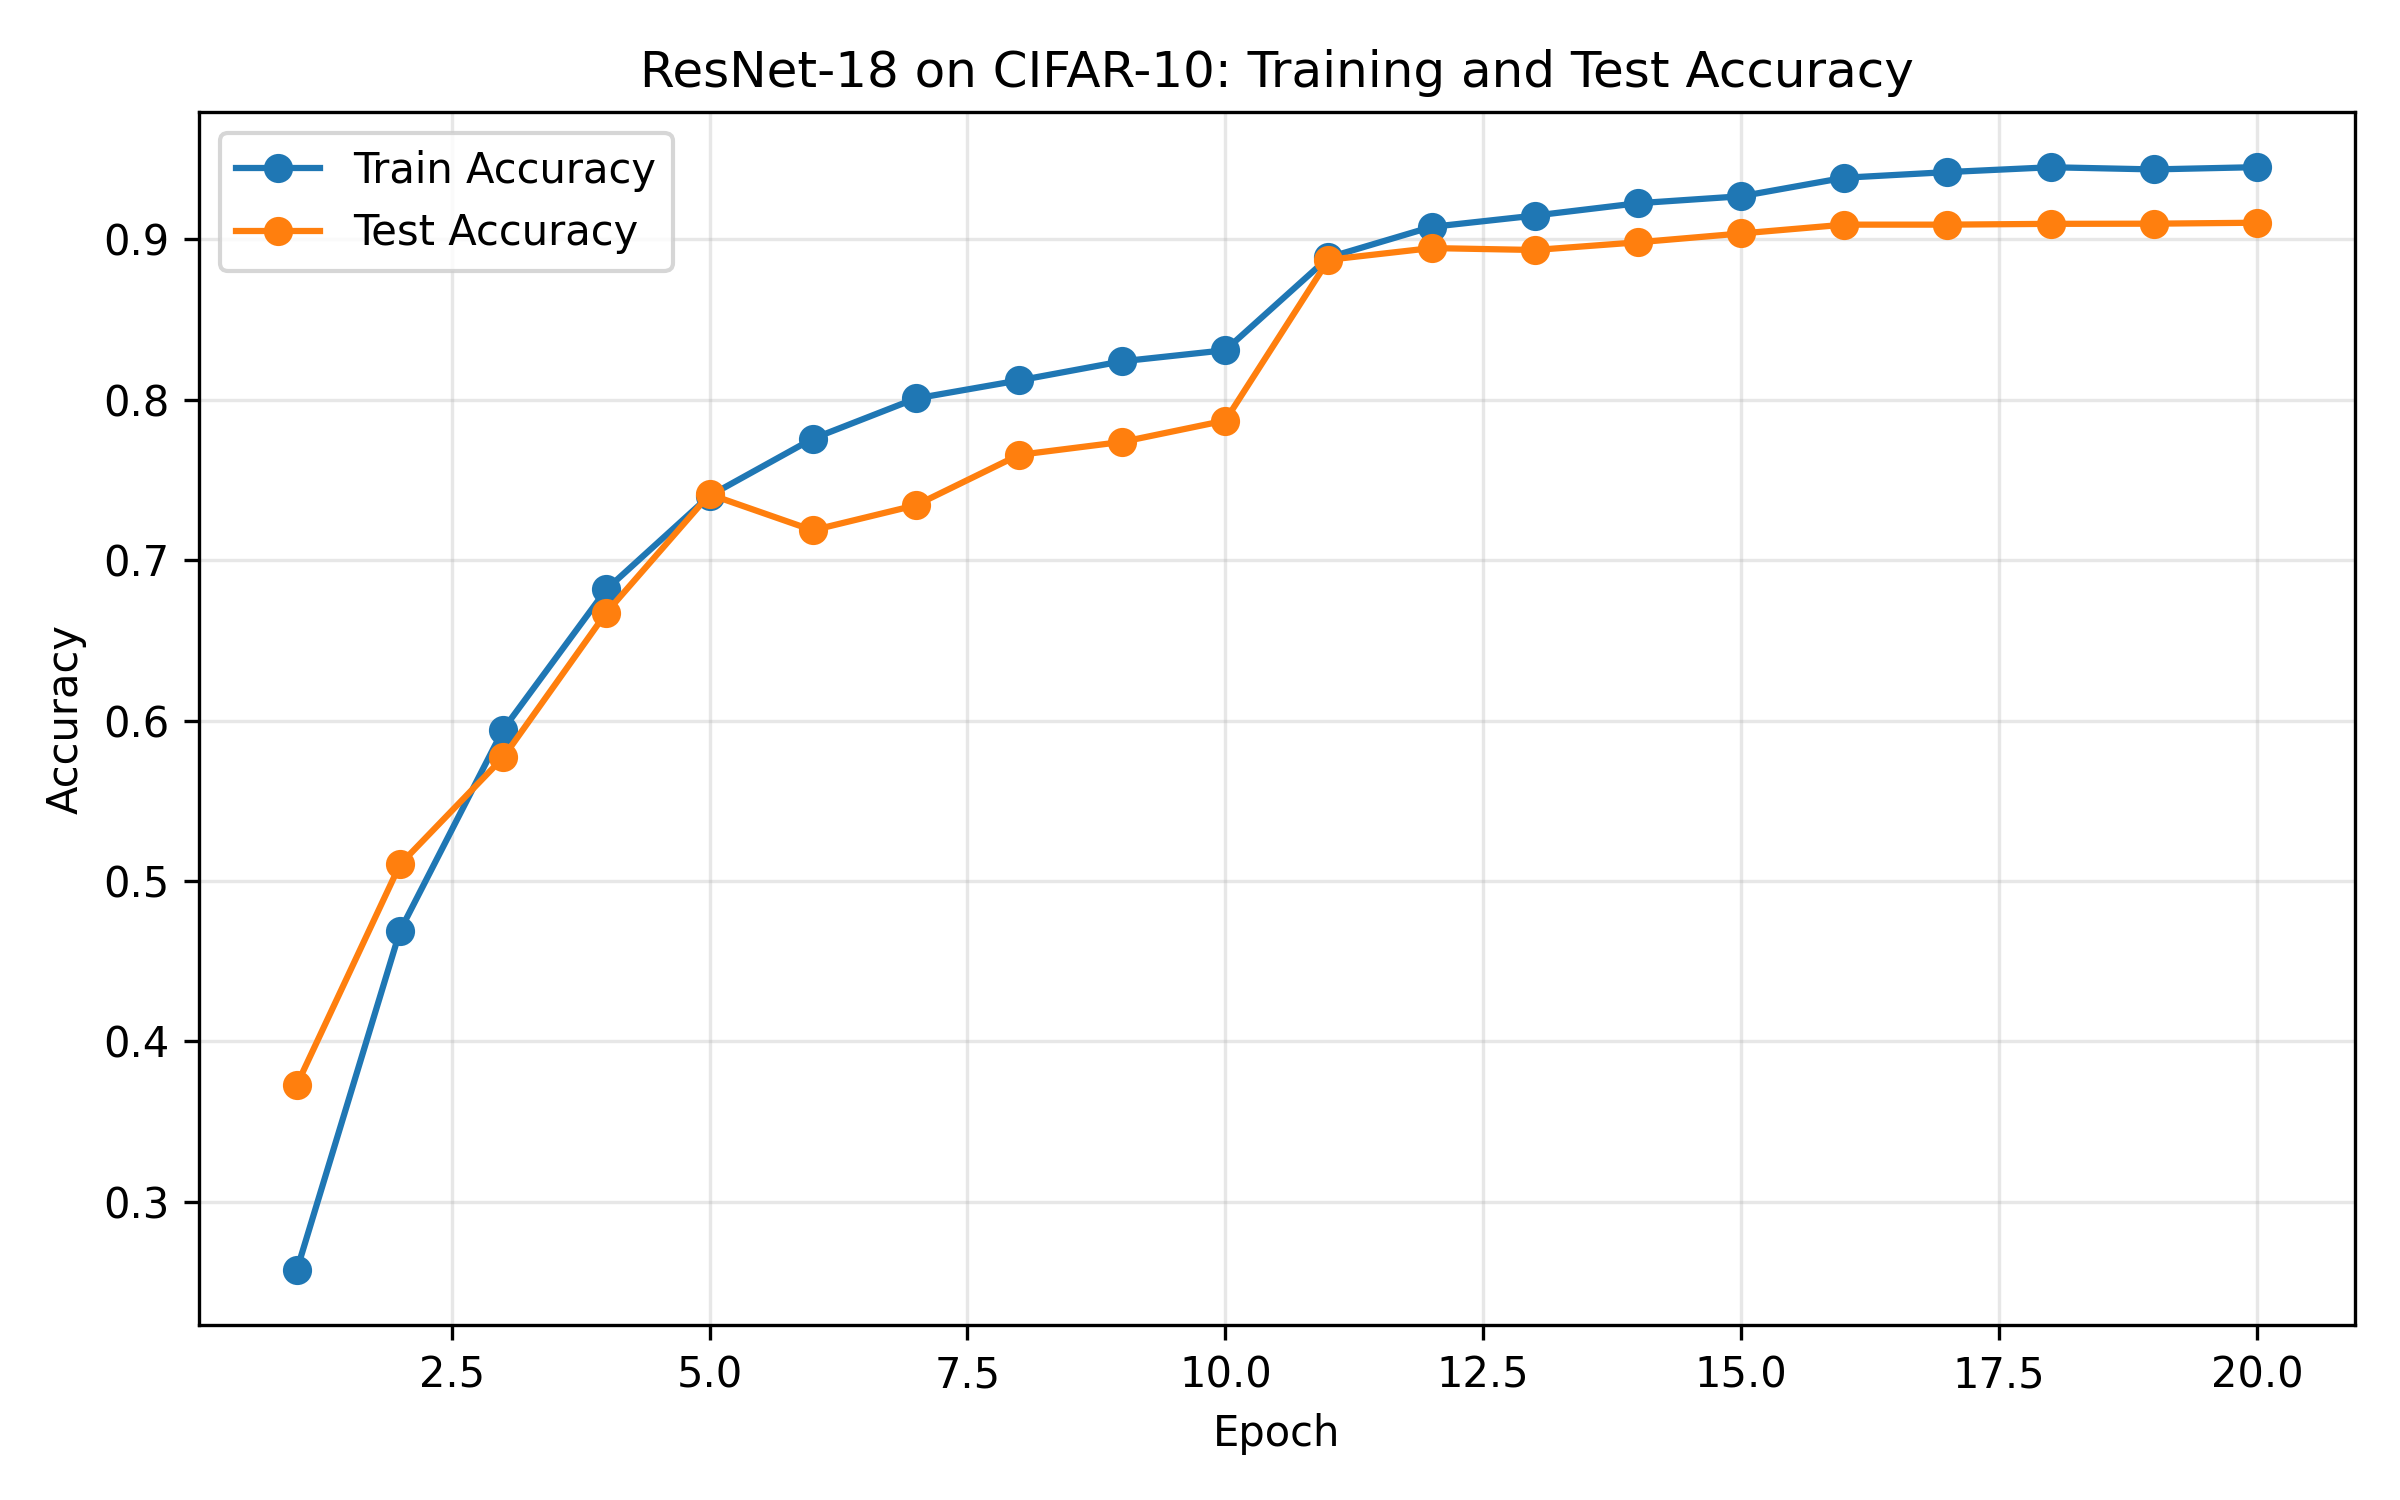
\includegraphics[width=\textwidth]{training_accuracy_resnet18_cifar10.png}
        \caption{Accuracy evolution.}
    \end{subfigure}
    \hfill
    \begin{subfigure}{0.48\textwidth}
        \centering
        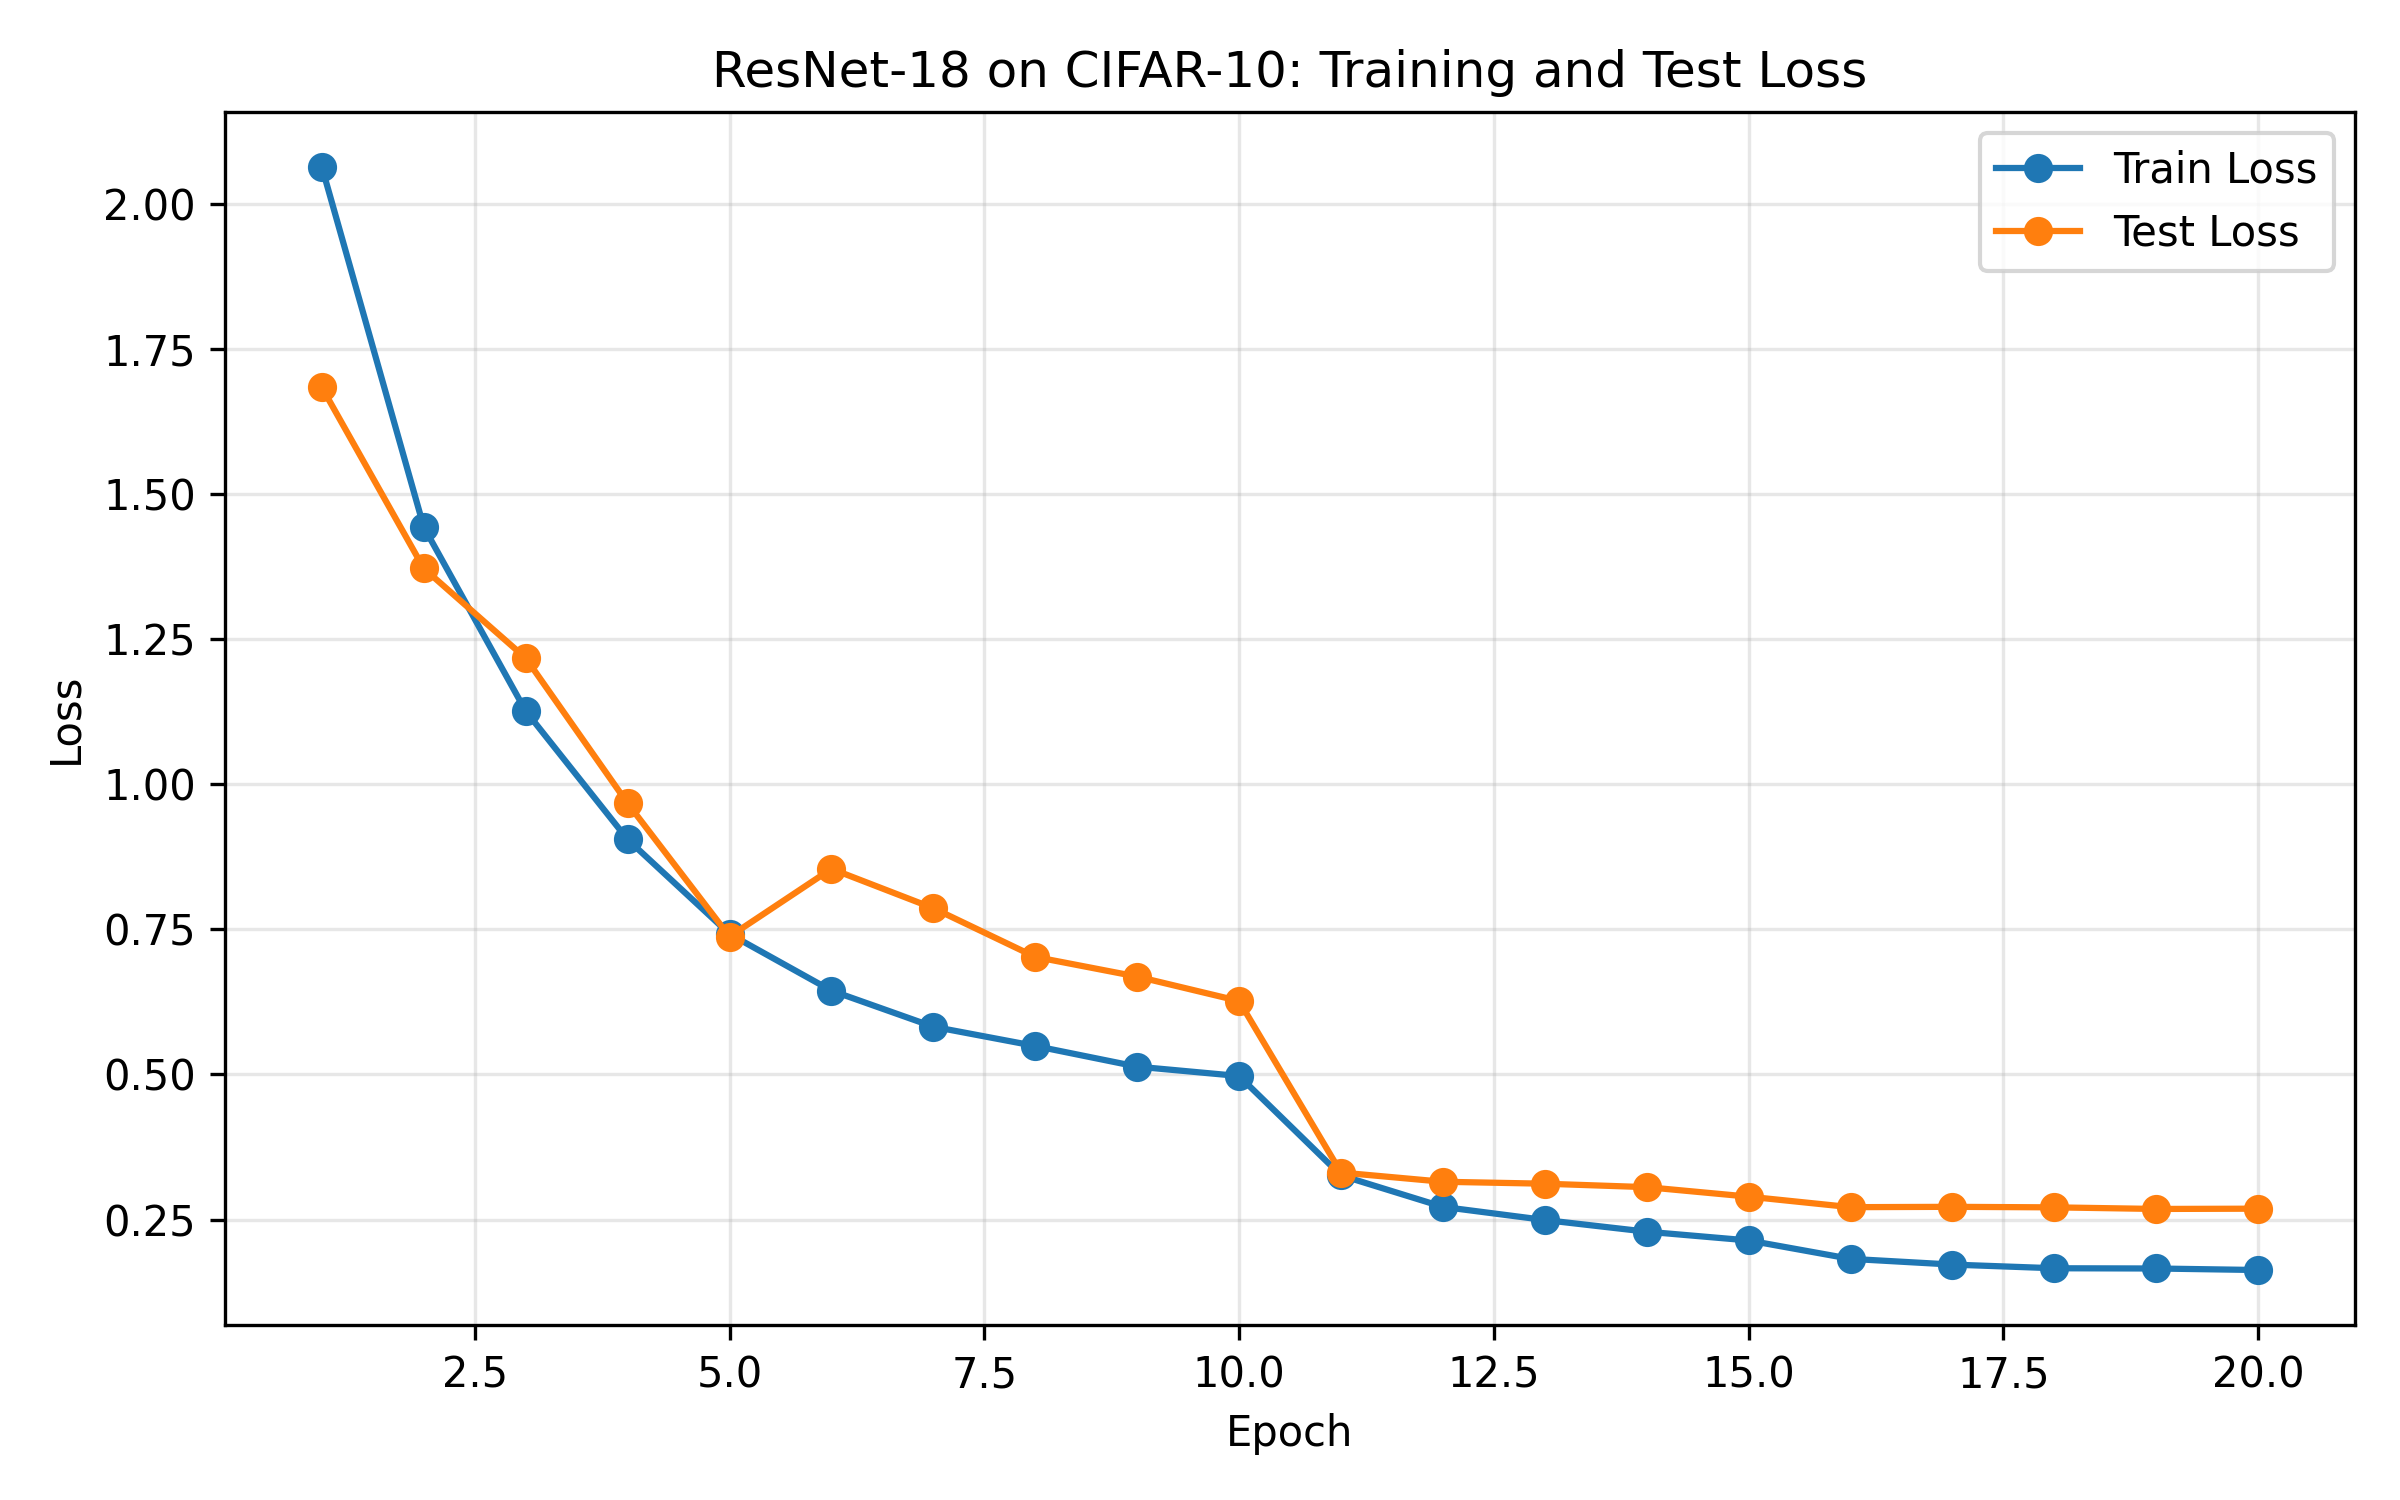
\includegraphics[width=\textwidth]{training_loss_resnet18_cifar10.png}
        \caption{Loss evolution.}
    \end{subfigure}
    \caption{Training history of the ResNet-18 model on CIFAR-10.}
    \label{fig:training}
\end{figure}

The best saved checkpoint reaches approximately $91.03\%$ test accuracy on CIFAR-10.
This model is then kept fixed for all OOD detection methods.

\section{Feature Extraction}

The Mahalanobis, KNN and simplified STOOD-X methods use the internal representation of the network.
For this purpose, the project defines a feature extractor that returns:

\begin{itemize}
    \item the penultimate-layer vector of the ResNet-18 model;
    \item the final logits of the classifier.
\end{itemize}

These features represent each image in a space learned by the model during CIFAR-10 training.
The central hypothesis is that ID images remain close to the training features, while OOD images tend to move away from that structure.

\section{OOD Detection Methods}

All methods follow the same experimental convention: high scores indicate that a sample is more likely to be ID, while low scores indicate that it is more likely to be OOD.

\subsection{Maximum Softmax Probability}

Maximum Softmax Probability (MSP) is a simple confidence-based baseline.
Given the logit vector $z(x)$, the softmax probability for class $c$ is:

\begin{equation}
    p(y=c \mid x) = \frac{\exp(z_c(x))}{\sum_j \exp(z_j(x))}.
\end{equation}

The MSP score is:

\begin{equation}
    s_{\text{MSP}}(x) = \max_c p(y=c \mid x).
\end{equation}

The intuition is that an ID image should produce higher maximum confidence than an OOD image.
The limitation is that neural networks can be overconfident on unknown inputs.

\subsection{Energy-based OOD Detection}

The Energy method uses the log-sum-exp function over the logits:

\begin{equation}
    E(x) = -T \log \sum_c \exp\left(\frac{z_c(x)}{T}\right),
\end{equation}

where $T$ is the temperature.
In this project, the returned score is $-E(x)$, in order to preserve the convention that high values indicate ID samples.
Unlike MSP, the Energy Score uses information from the full logit vector, not only the largest probability.

\subsection{ODIN}

ODIN combines two ideas:

\begin{itemize}
    \item temperature scaling, which modifies the softmax distribution;
    \item a small input perturbation, computed from the gradient, to increase the separability between ID and OOD samples.
\end{itemize}

The project uses $T=1000$ and $\epsilon=0.001$.
After the perturbation, the score is again the maximum softmax probability.
ODIN is a post-hoc method because it does not require retraining the network.

\subsection{Mahalanobis}

The Mahalanobis method operates in feature space.
For each CIFAR-10 class, the mean of the training features is computed:

\begin{equation}
    \mu_c = \frac{1}{N_c}\sum_{i:y_i=c} f(x_i).
\end{equation}

A global covariance matrix $\Sigma$ is then estimated.
The Mahalanobis distance between a sample and a class is:

\begin{equation}
    d_c(x) = (f(x)-\mu_c)^T\Sigma^{-1}(f(x)-\mu_c).
\end{equation}

The score is the negative minimum distance:

\begin{equation}
    s_{\text{Mahalanobis}}(x) = -\min_c d_c(x).
\end{equation}

Thus, a sample that is close to one of the ID classes receives a high score.

\subsection{KNN}

The KNN method also uses penultimate-layer features.
First, all CIFAR-10 training features are stored as a reference bank.
For each test image, the distance to the ID feature bank is computed and the distance to the $k$-th nearest neighbor is selected.

The score is:

\begin{equation}
    s_{\text{KNN}}(x) = -d_k(f(x), \mathcal{F}_{\text{train}}),
\end{equation}

where $d_k$ is the distance to the $k$-th neighbor and $\mathcal{F}_{\text{train}}$ is the set of ID training features.
In this project, $k=50$.
Features are normalized before distances are computed.

\subsection{Simplified STOOD-X}

The STOOD-X paper proposes a two-stage methodology~\cite{stoodx2025}.
The first stage is an OOD detector based on feature-space distances and a nonparametric statistical test, the Wilcoxon-Mann-Whitney test.
The second stage adds user-oriented visual explainability, aligned with the BLUE XAI perspective.

In this project, this methodology was replicated only partially.
The replication preserves the fundamental idea of comparing a new sample with the ID distribution in feature space, but simplifies the statistical procedure.
Instead of directly applying the Wilcoxon-Mann-Whitney test used in the original paper, the project uses an empirical distribution of KNN distances obtained from CIFAR-10 training features.

The implemented method can be seen as a practical and reduced version of the first stage of STOOD-X.
The procedure is:

\begin{enumerate}
    \item extract features from the CIFAR-10 training set;
    \item compute, for each ID training sample, the distance to its $k$-th nearest neighbor;
    \item build a reference distribution of ID distances;
    \item compute the KNN distance of each new sample;
    \item transform that distance into an empirical p-value.
\end{enumerate}

The empirical p-value is computed as:

\begin{equation}
    p(x) = \frac{1}{N}\sum_{i=1}^{N}\mathbb{I}(d_i^{\text{ref}} \geq d(x)).
\end{equation}

If a sample has a small distance to the ID bank, many reference distances will be larger than its distance.
In that case, the p-value is high and the sample is considered similar to the ID distribution.
If the distance is large, the p-value is low and the sample is more likely to be OOD.

This approximation makes it possible to experimentally test the main motivation behind STOOD-X: OOD samples should behave statistically differently in feature space when compared with ID samples.
However, since this is a simplified replication, the results should not be interpreted as an exact reproduction of the results reported in the original paper.

\section{Evaluation Metrics}

Four metrics were used:

\begin{itemize}
    \item \textbf{AUROC}: area under the ROC curve. Higher is better.
    \item \textbf{AUPR-IN}: area under the precision-recall curve when ID is treated as the positive class.
    \item \textbf{AUPR-OUT}: area under the precision-recall curve when OOD is treated as the positive class.
    \item \textbf{FPR95}: false positive rate when the true positive rate is close to 95\%. Lower is better.
\end{itemize}

In the implementation, ID samples are assigned label 1 and OOD samples are assigned label 0.
Since all methods follow the convention that high scores indicate ID samples, the same metric implementation can be used for every method.

\section{Experimental Pipeline}

The main pipeline runs the complete experiment.
The steps are:

\begin{enumerate}
    \item clean previous results and checkpoints;
    \item train the ResNet-18 model on CIFAR-10;
    \item generate training curves;
    \item evaluate MSP, Energy, Mahalanobis, KNN, ODIN and STOOD-X individually;
    \item combine the results;
    \item create rankings by AUROC and FPR95;
    \item generate the final table;
    \item create comparative plots, heatmaps, boxplots, ROC curves, score histograms, t-SNE, UMAP and a confusion matrix.
\end{enumerate}

The main outputs are stored in:

\begin{itemize}
    \item \texttt{results/tables/};
    \item \texttt{results/figures/};
    \item \texttt{results/roc\_curves/};
    \item \texttt{results/score\_distributions/};
    \item \texttt{results/tsne\_umap/};
    \item \texttt{results/confusion\_matrices/}.
\end{itemize}

\section{Results}

\subsection{Quantitative Results}

Table~\ref{tab:results} presents the final results.
For AUROC, AUPR-IN and AUPR-OUT, higher values are better.
For FPR95, lower values are better.

\begin{table}[H]
\centering
\caption{Final OOD detection results.}
\label{tab:results}
\small
\resizebox{\textwidth}{!}{
\begin{tabular}{llrrrr}
\toprule
Method & OOD Dataset & AUROC & AUPR-IN & AUPR-OUT & FPR95 \\
\midrule
ODIN & CIFAR100 & 0.8810 & 0.8916 & 0.8587 & 0.5838 \\
Energy & CIFAR100 & 0.8807 & 0.8913 & 0.8576 & 0.5825 \\
KNN & CIFAR100 & 0.8707 & 0.8814 & 0.8506 & 0.6001 \\
STOOD-X & CIFAR100 & 0.8706 & 0.8814 & 0.8507 & 0.6003 \\
MSP & CIFAR100 & 0.8543 & 0.8773 & 0.8189 & 0.7125 \\
Mahalanobis & CIFAR100 & 0.5495 & 0.5641 & 0.5334 & 0.9386 \\
\midrule
ODIN & MNIST & 0.9643 & 0.9709 & 0.9561 & 0.2211 \\
Energy & MNIST & 0.9638 & 0.9706 & 0.9536 & 0.2073 \\
STOOD-X & MNIST & 0.9551 & 0.9611 & 0.9447 & 0.2380 \\
KNN & MNIST & 0.9549 & 0.9611 & 0.9441 & 0.2432 \\
MSP & MNIST & 0.9045 & 0.9235 & 0.8826 & 0.5599 \\
Mahalanobis & MNIST & 0.3234 & 0.4127 & 0.3889 & 0.9845 \\
\midrule
STOOD-X & SVHN & 0.9339 & 0.9094 & 0.9578 & 0.4916 \\
KNN & SVHN & 0.9333 & 0.9094 & 0.9568 & 0.5035 \\
ODIN & SVHN & 0.9168 & 0.8913 & 0.9400 & 0.6110 \\
Energy & SVHN & 0.9101 & 0.8856 & 0.9314 & 0.6549 \\
MSP & SVHN & 0.8923 & 0.8671 & 0.9293 & 0.7090 \\
Mahalanobis & SVHN & 0.7626 & 0.6031 & 0.8730 & 0.7886 \\
\bottomrule
\end{tabular}
}
\end{table}

\subsection{Global Comparison}

On CIFAR-100, ODIN obtains the best AUROC, with Energy almost tied.
Energy obtains the best FPR95 on this dataset.
Since CIFAR-100 is visually close to CIFAR-10, this is a more difficult scenario than MNIST.

On MNIST, ODIN and Energy obtain the best results.
This is expected, because MNIST is very different from CIFAR-10.
Even so, KNN and the simplified STOOD-X method also achieve strong performance.

On SVHN, the best methods are STOOD-X and KNN.
This suggests that, in this case, the geometry of the feature space is more informative than scores directly derived from logits.

\begin{figure}[H]
    \centering
    \begin{subfigure}{0.48\textwidth}
        \centering
        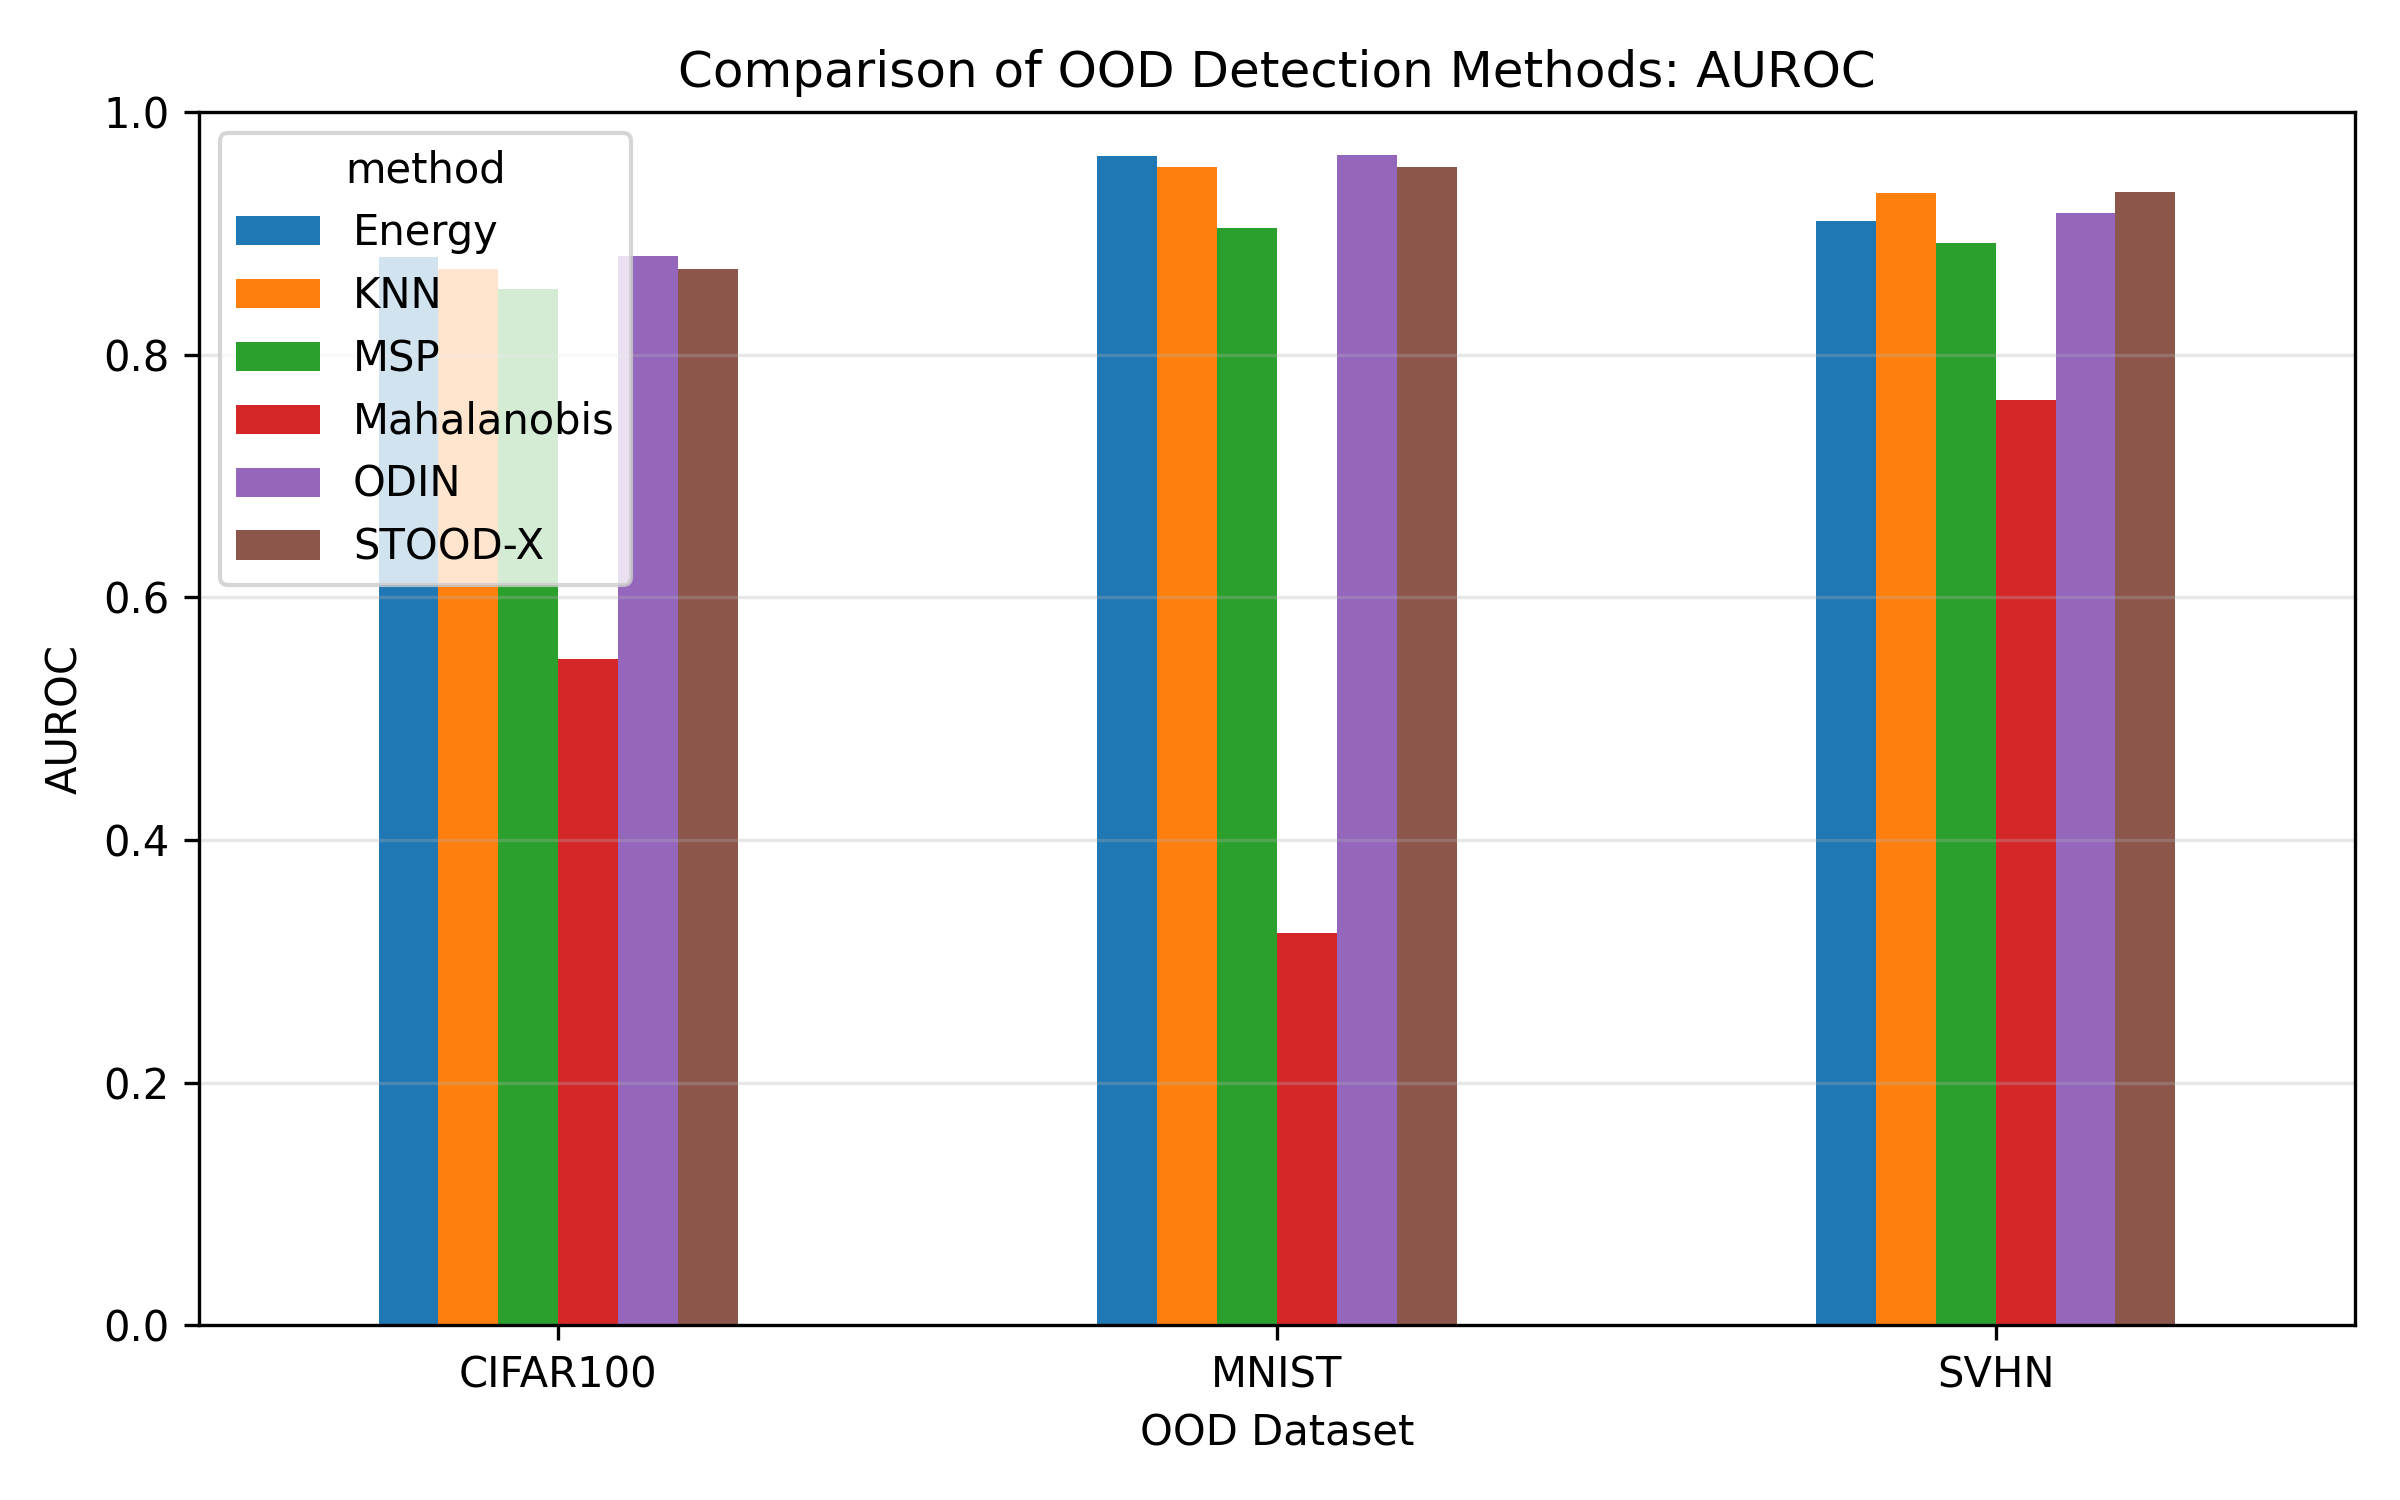
\includegraphics[width=\textwidth]{comparison_methods_auroc.png}
        \caption{AUROC comparison.}
    \end{subfigure}
    \hfill
    \begin{subfigure}{0.48\textwidth}
        \centering
        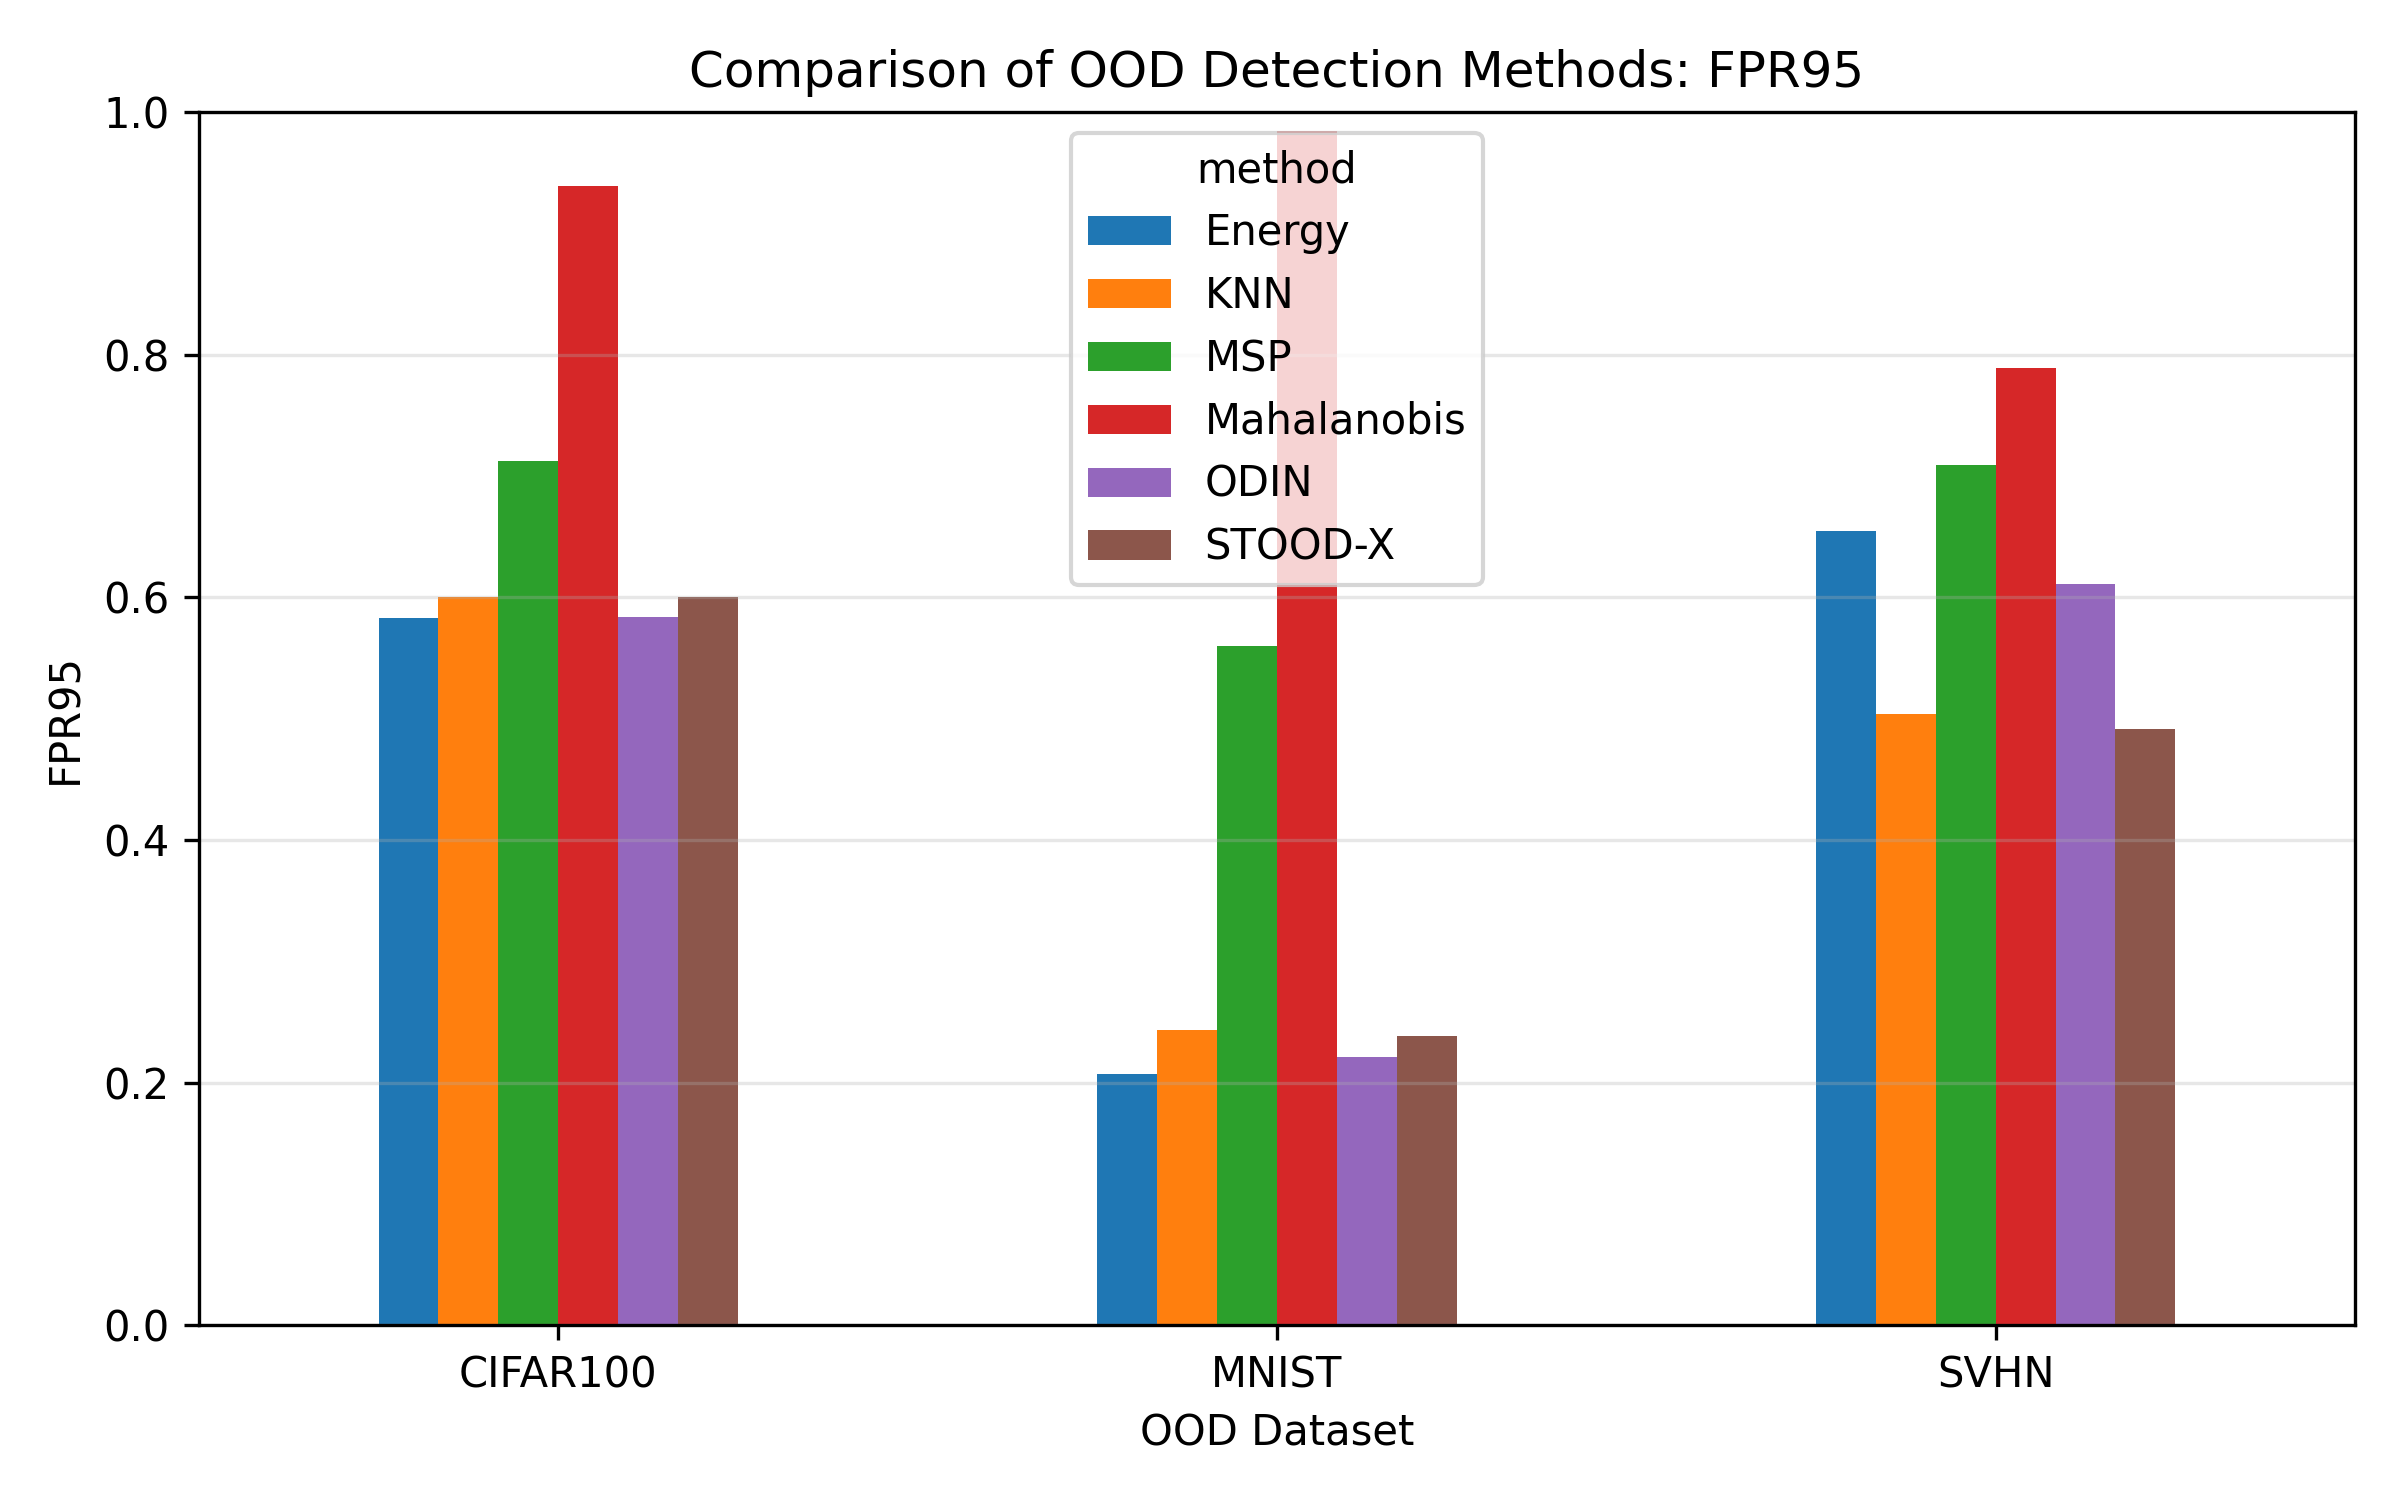
\includegraphics[width=\textwidth]{comparison_methods_fpr95.png}
        \caption{FPR95 comparison.}
    \end{subfigure}
    \caption{Global comparison of OOD detection methods.}
    \label{fig:global-comparison}
\end{figure}

\begin{figure}[H]
    \centering
    \begin{subfigure}{0.48\textwidth}
        \centering
        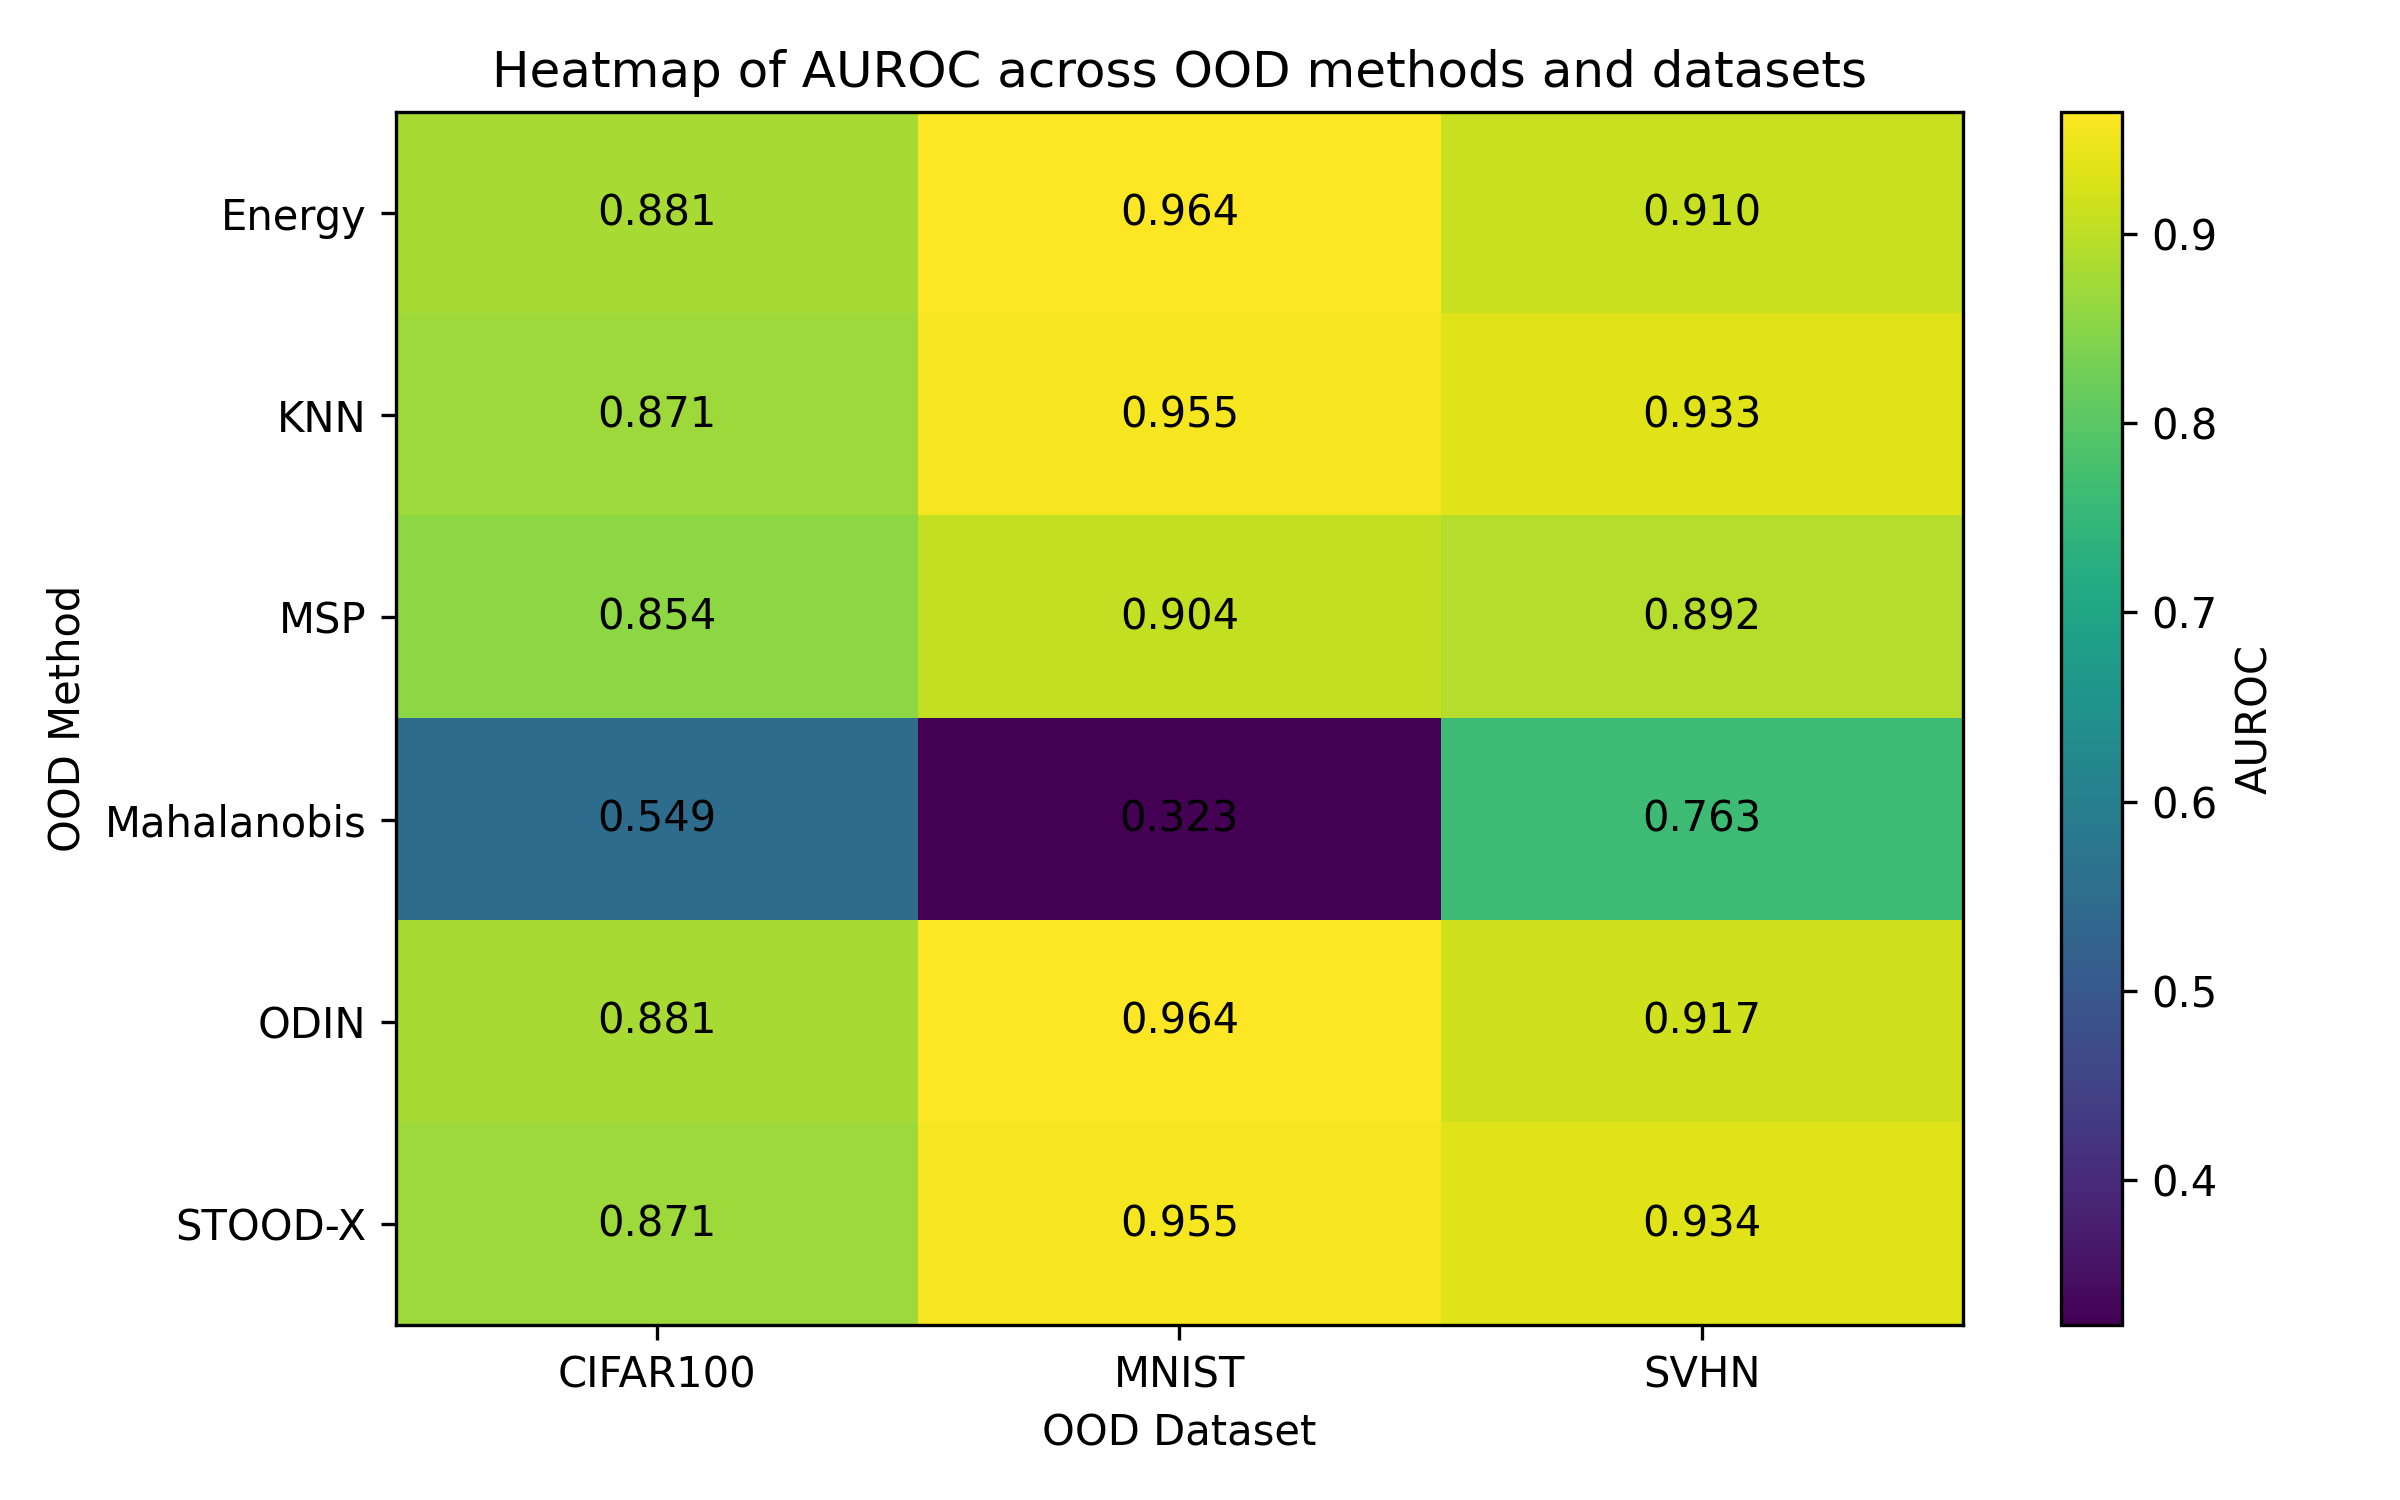
\includegraphics[width=\textwidth]{heatmap_auroc_methods_datasets.png}
        \caption{AUROC heatmap.}
    \end{subfigure}
    \hfill
    \begin{subfigure}{0.48\textwidth}
        \centering
        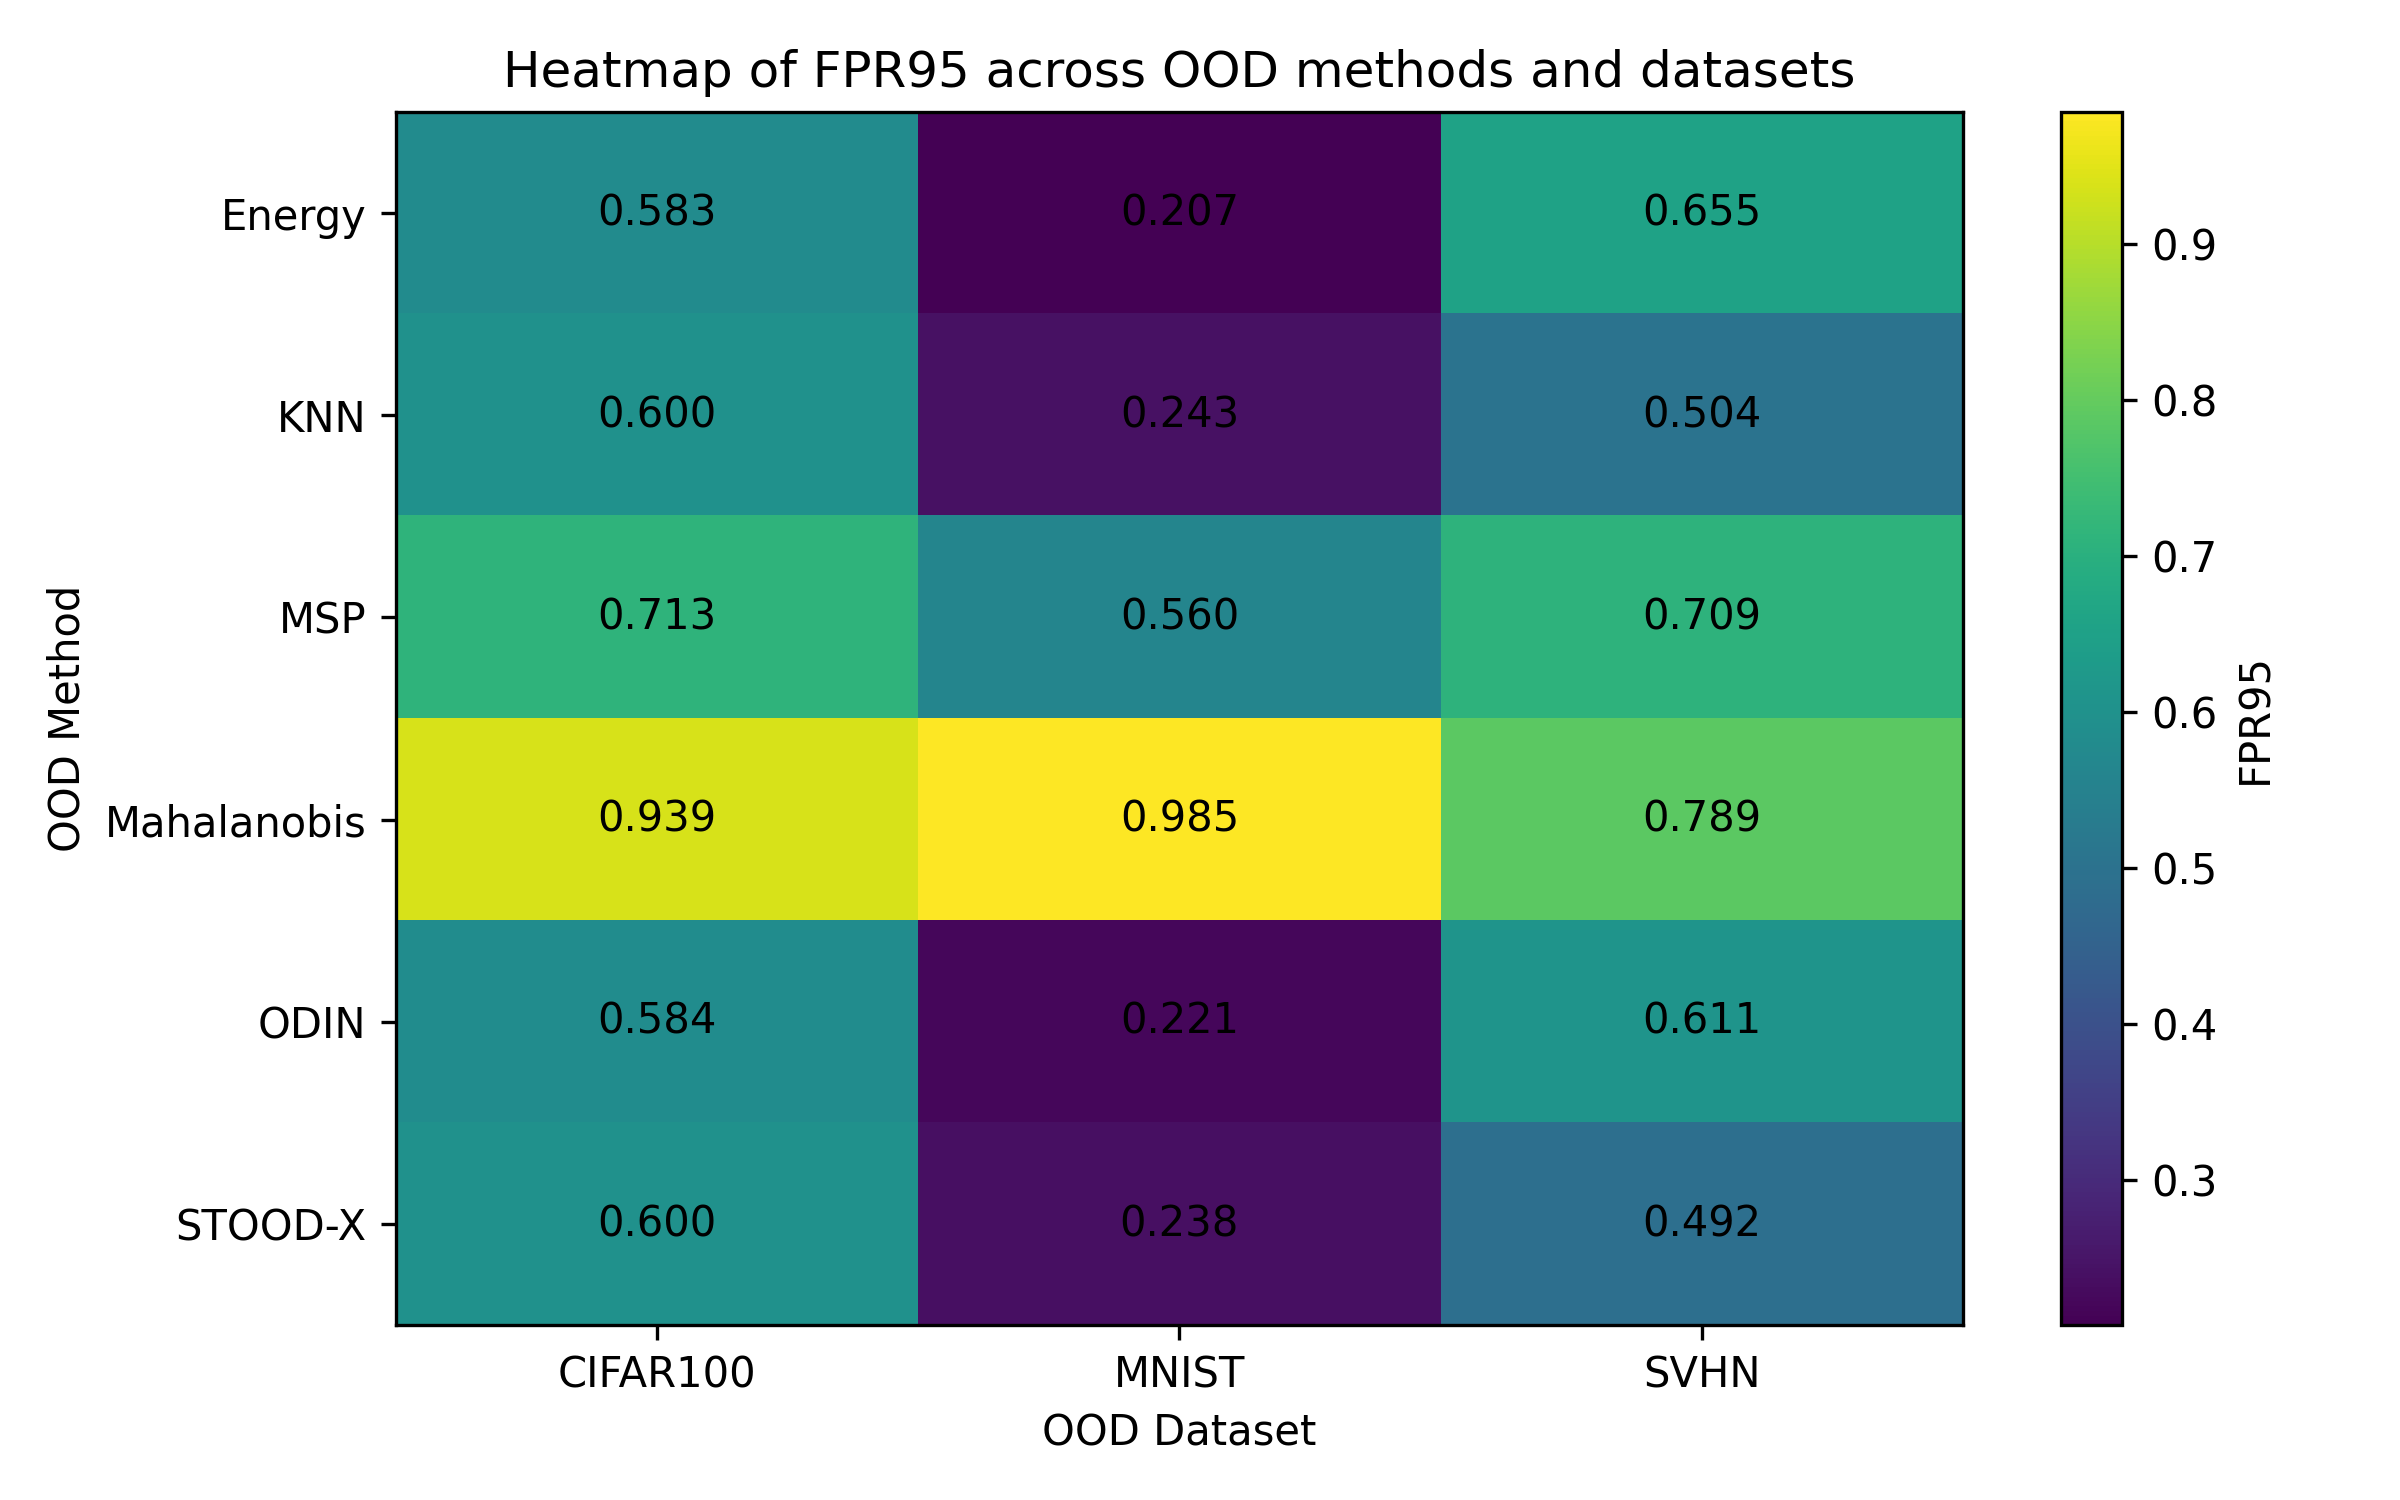
\includegraphics[width=\textwidth]{heatmap_fpr95_methods_datasets.png}
        \caption{FPR95 heatmap.}
    \end{subfigure}
    \caption{Heatmaps of results by method and OOD dataset.}
    \label{fig:heatmaps}
\end{figure}

\subsection{Score Distributions}

The score histograms make it possible to directly observe the separation between ID and OOD samples.
A good detector should assign high scores to CIFAR-10 samples and lower scores to OOD samples.
When the distributions overlap strongly, the method has difficulty separating the two groups.

\begin{figure}[H]
    \centering
    \begin{subfigure}{0.32\textwidth}
        \centering
        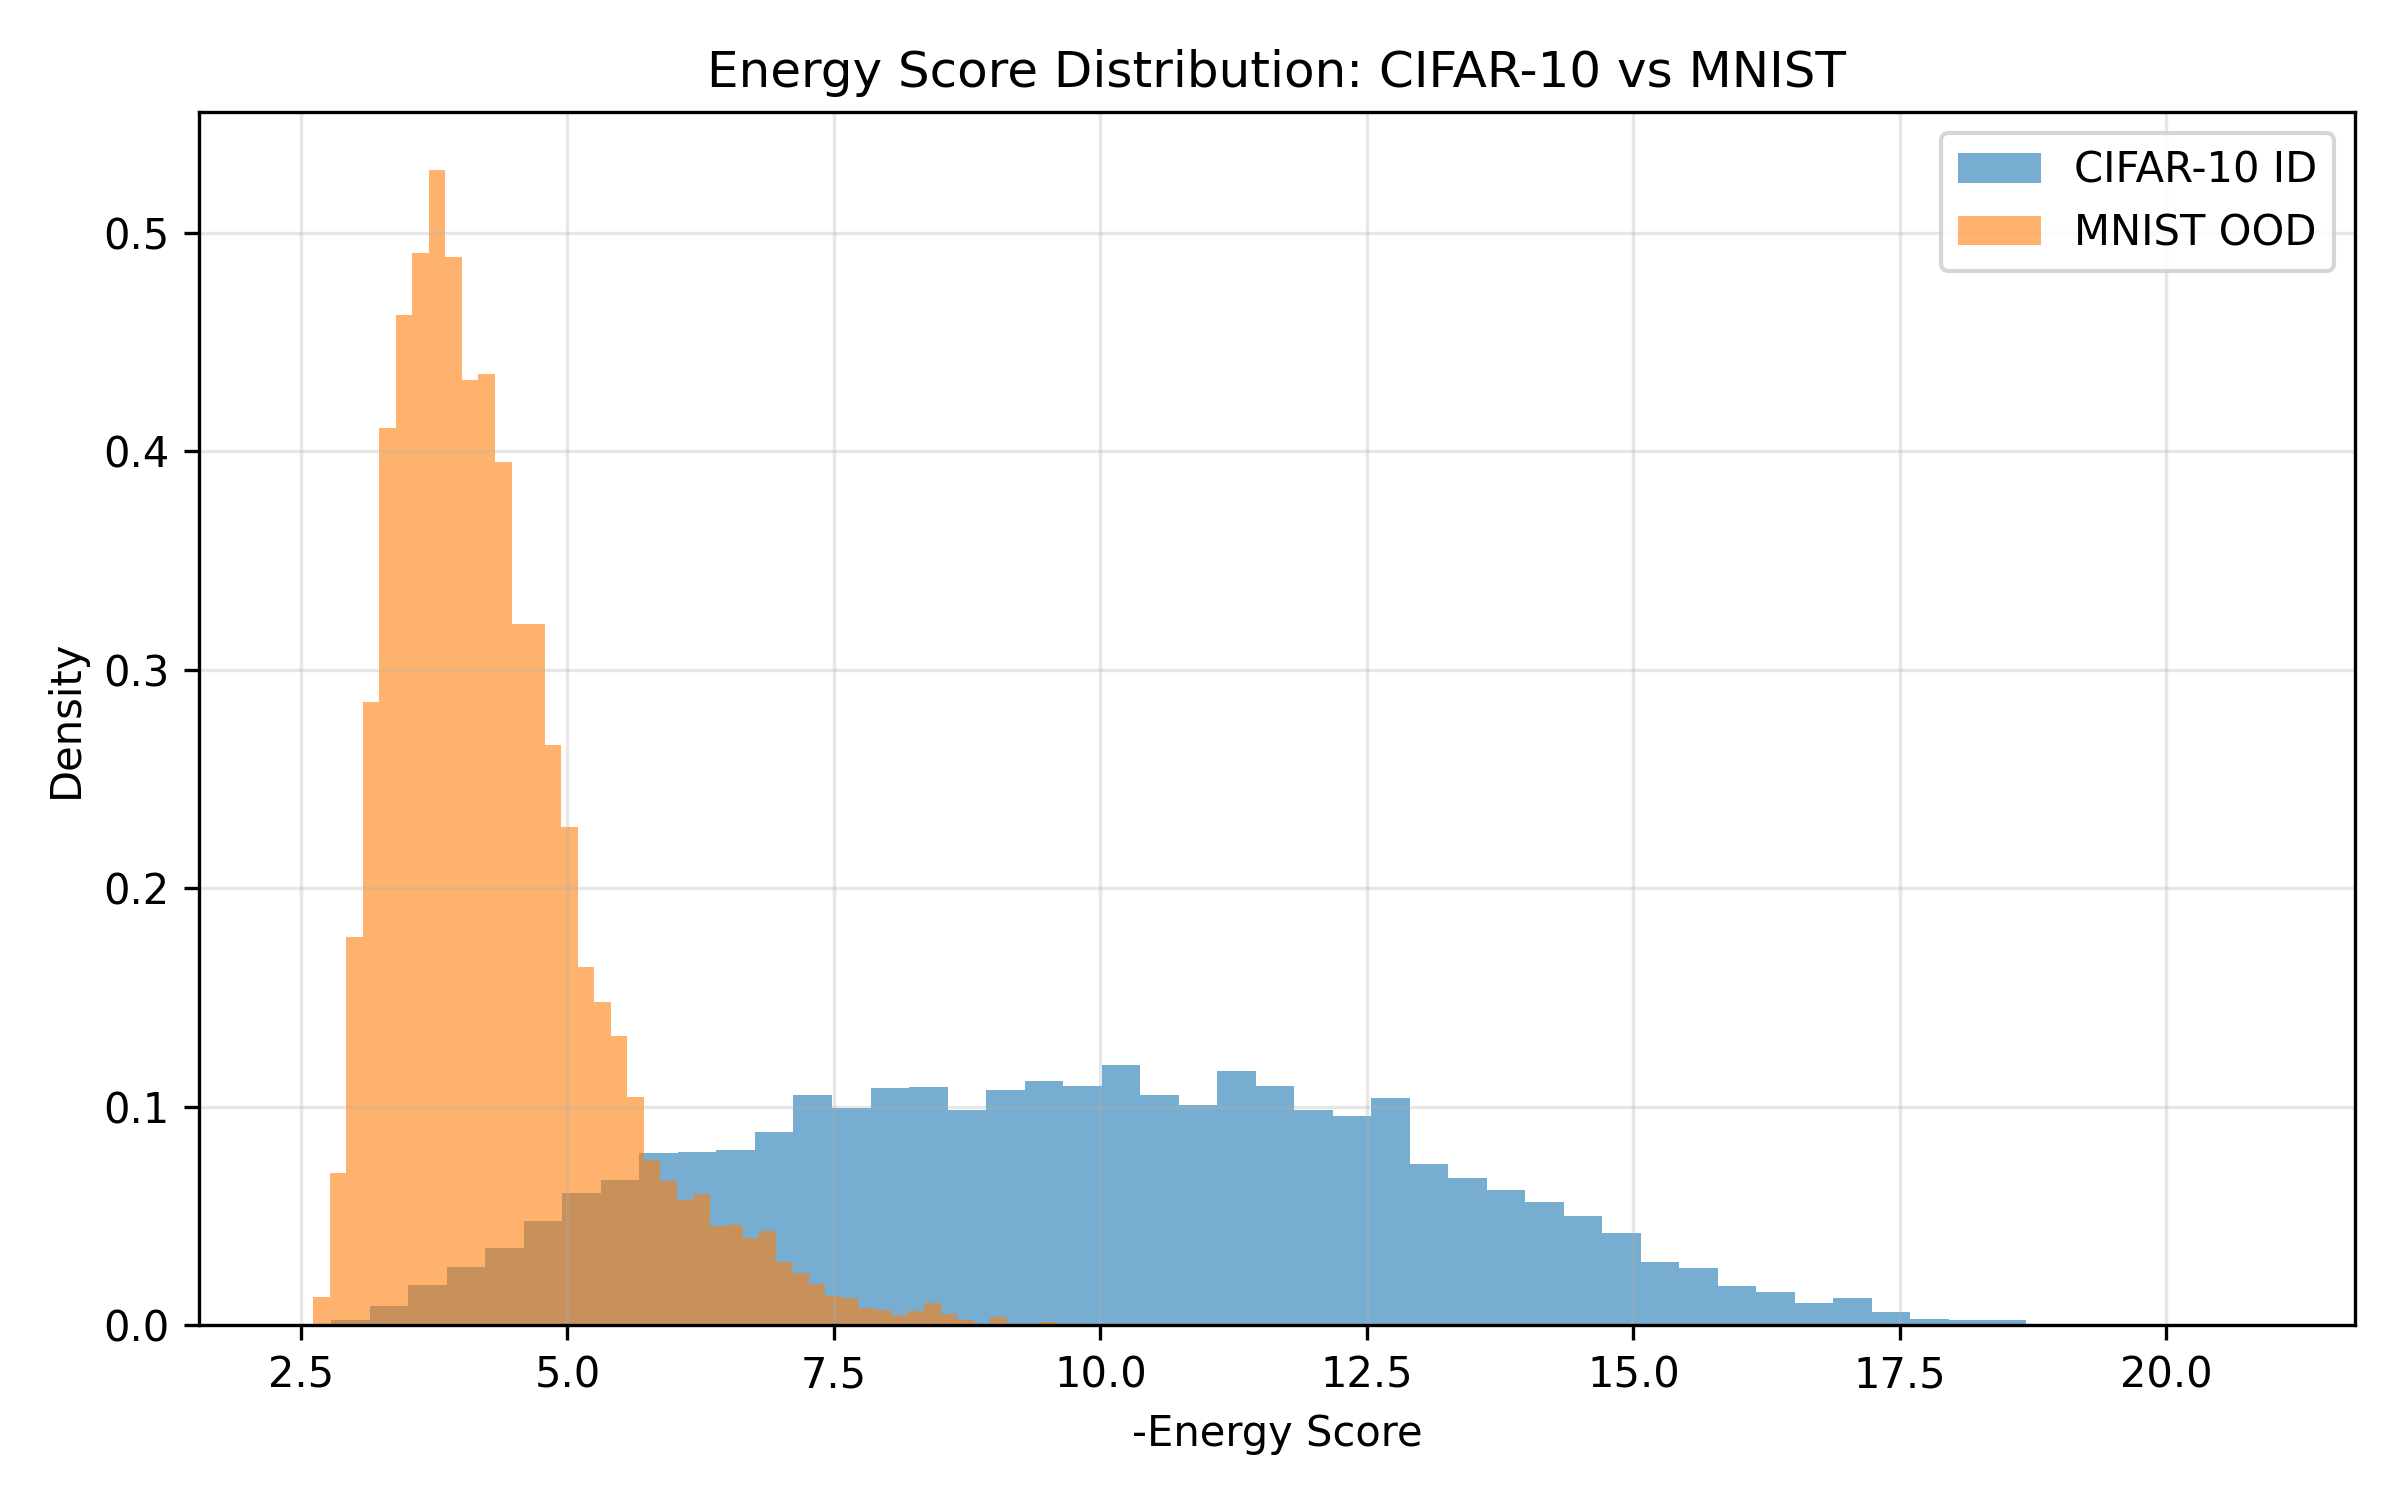
\includegraphics[width=\textwidth]{energy_cifar10_vs_mnist.png}
        \caption{Energy on MNIST.}
    \end{subfigure}
    \hfill
    \begin{subfigure}{0.32\textwidth}
        \centering
        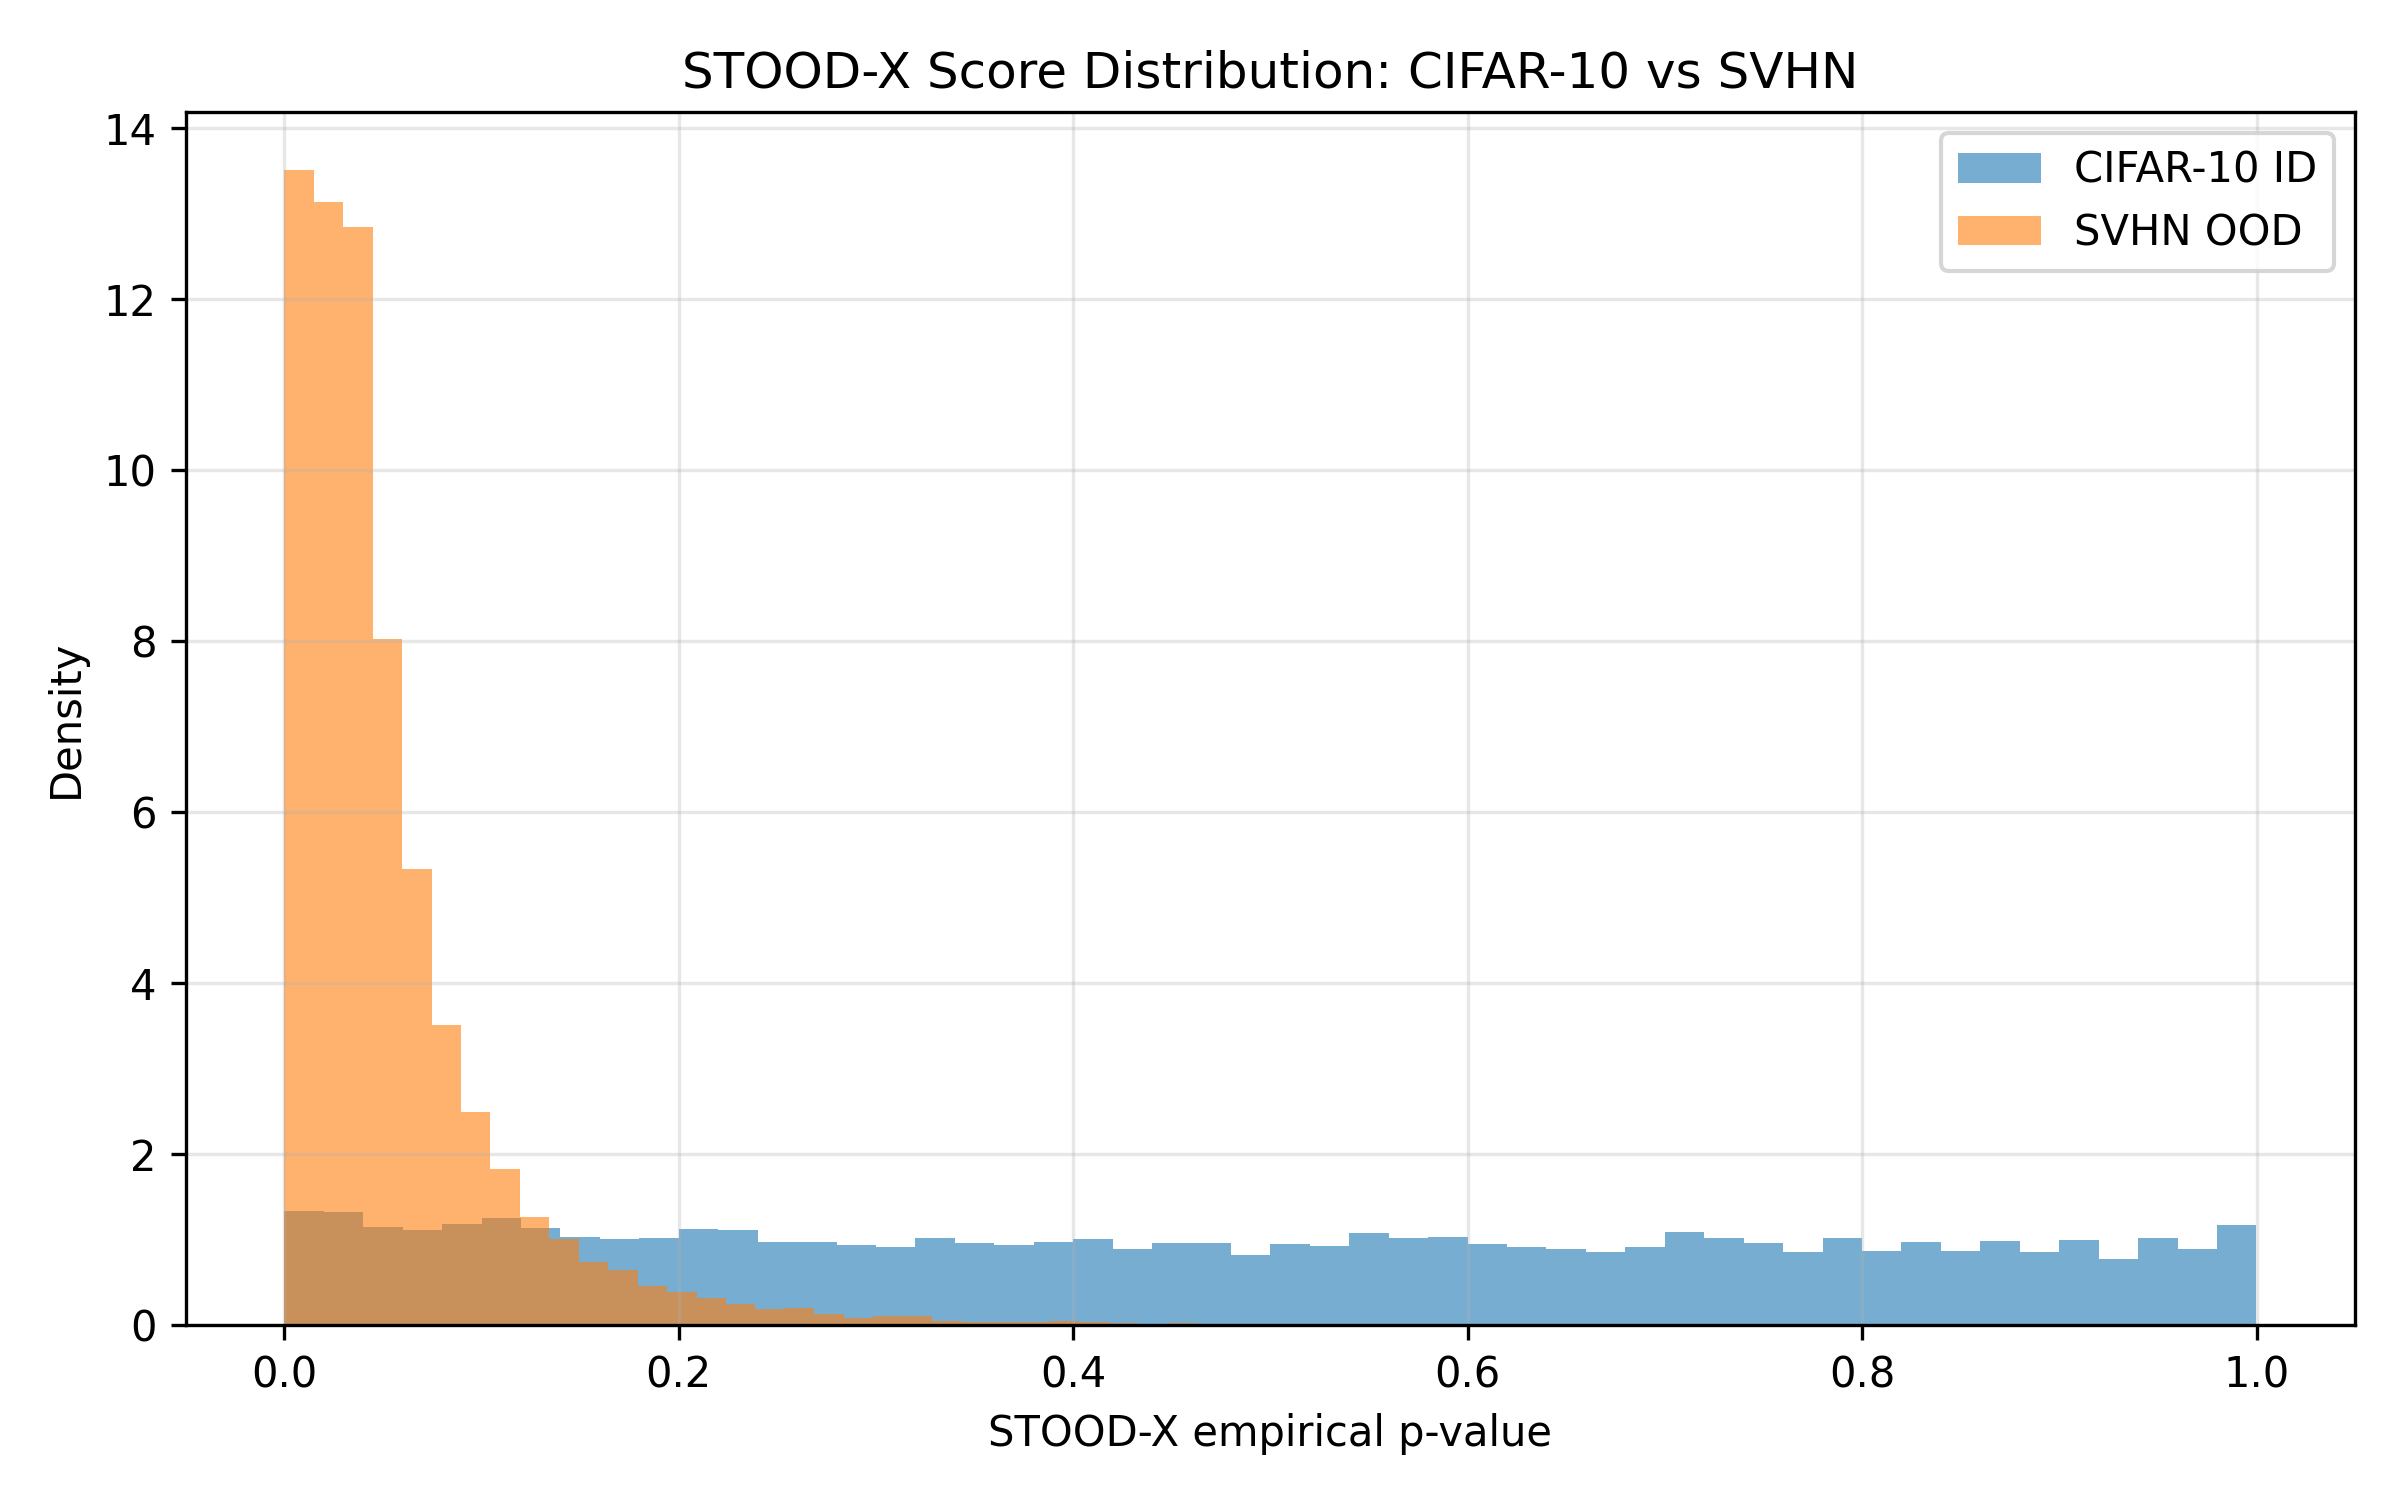
\includegraphics[width=\textwidth]{stoodx_cifar10_vs_svhn.png}
        \caption{STOOD-X on SVHN.}
    \end{subfigure}
    \hfill
    \begin{subfigure}{0.32\textwidth}
        \centering
        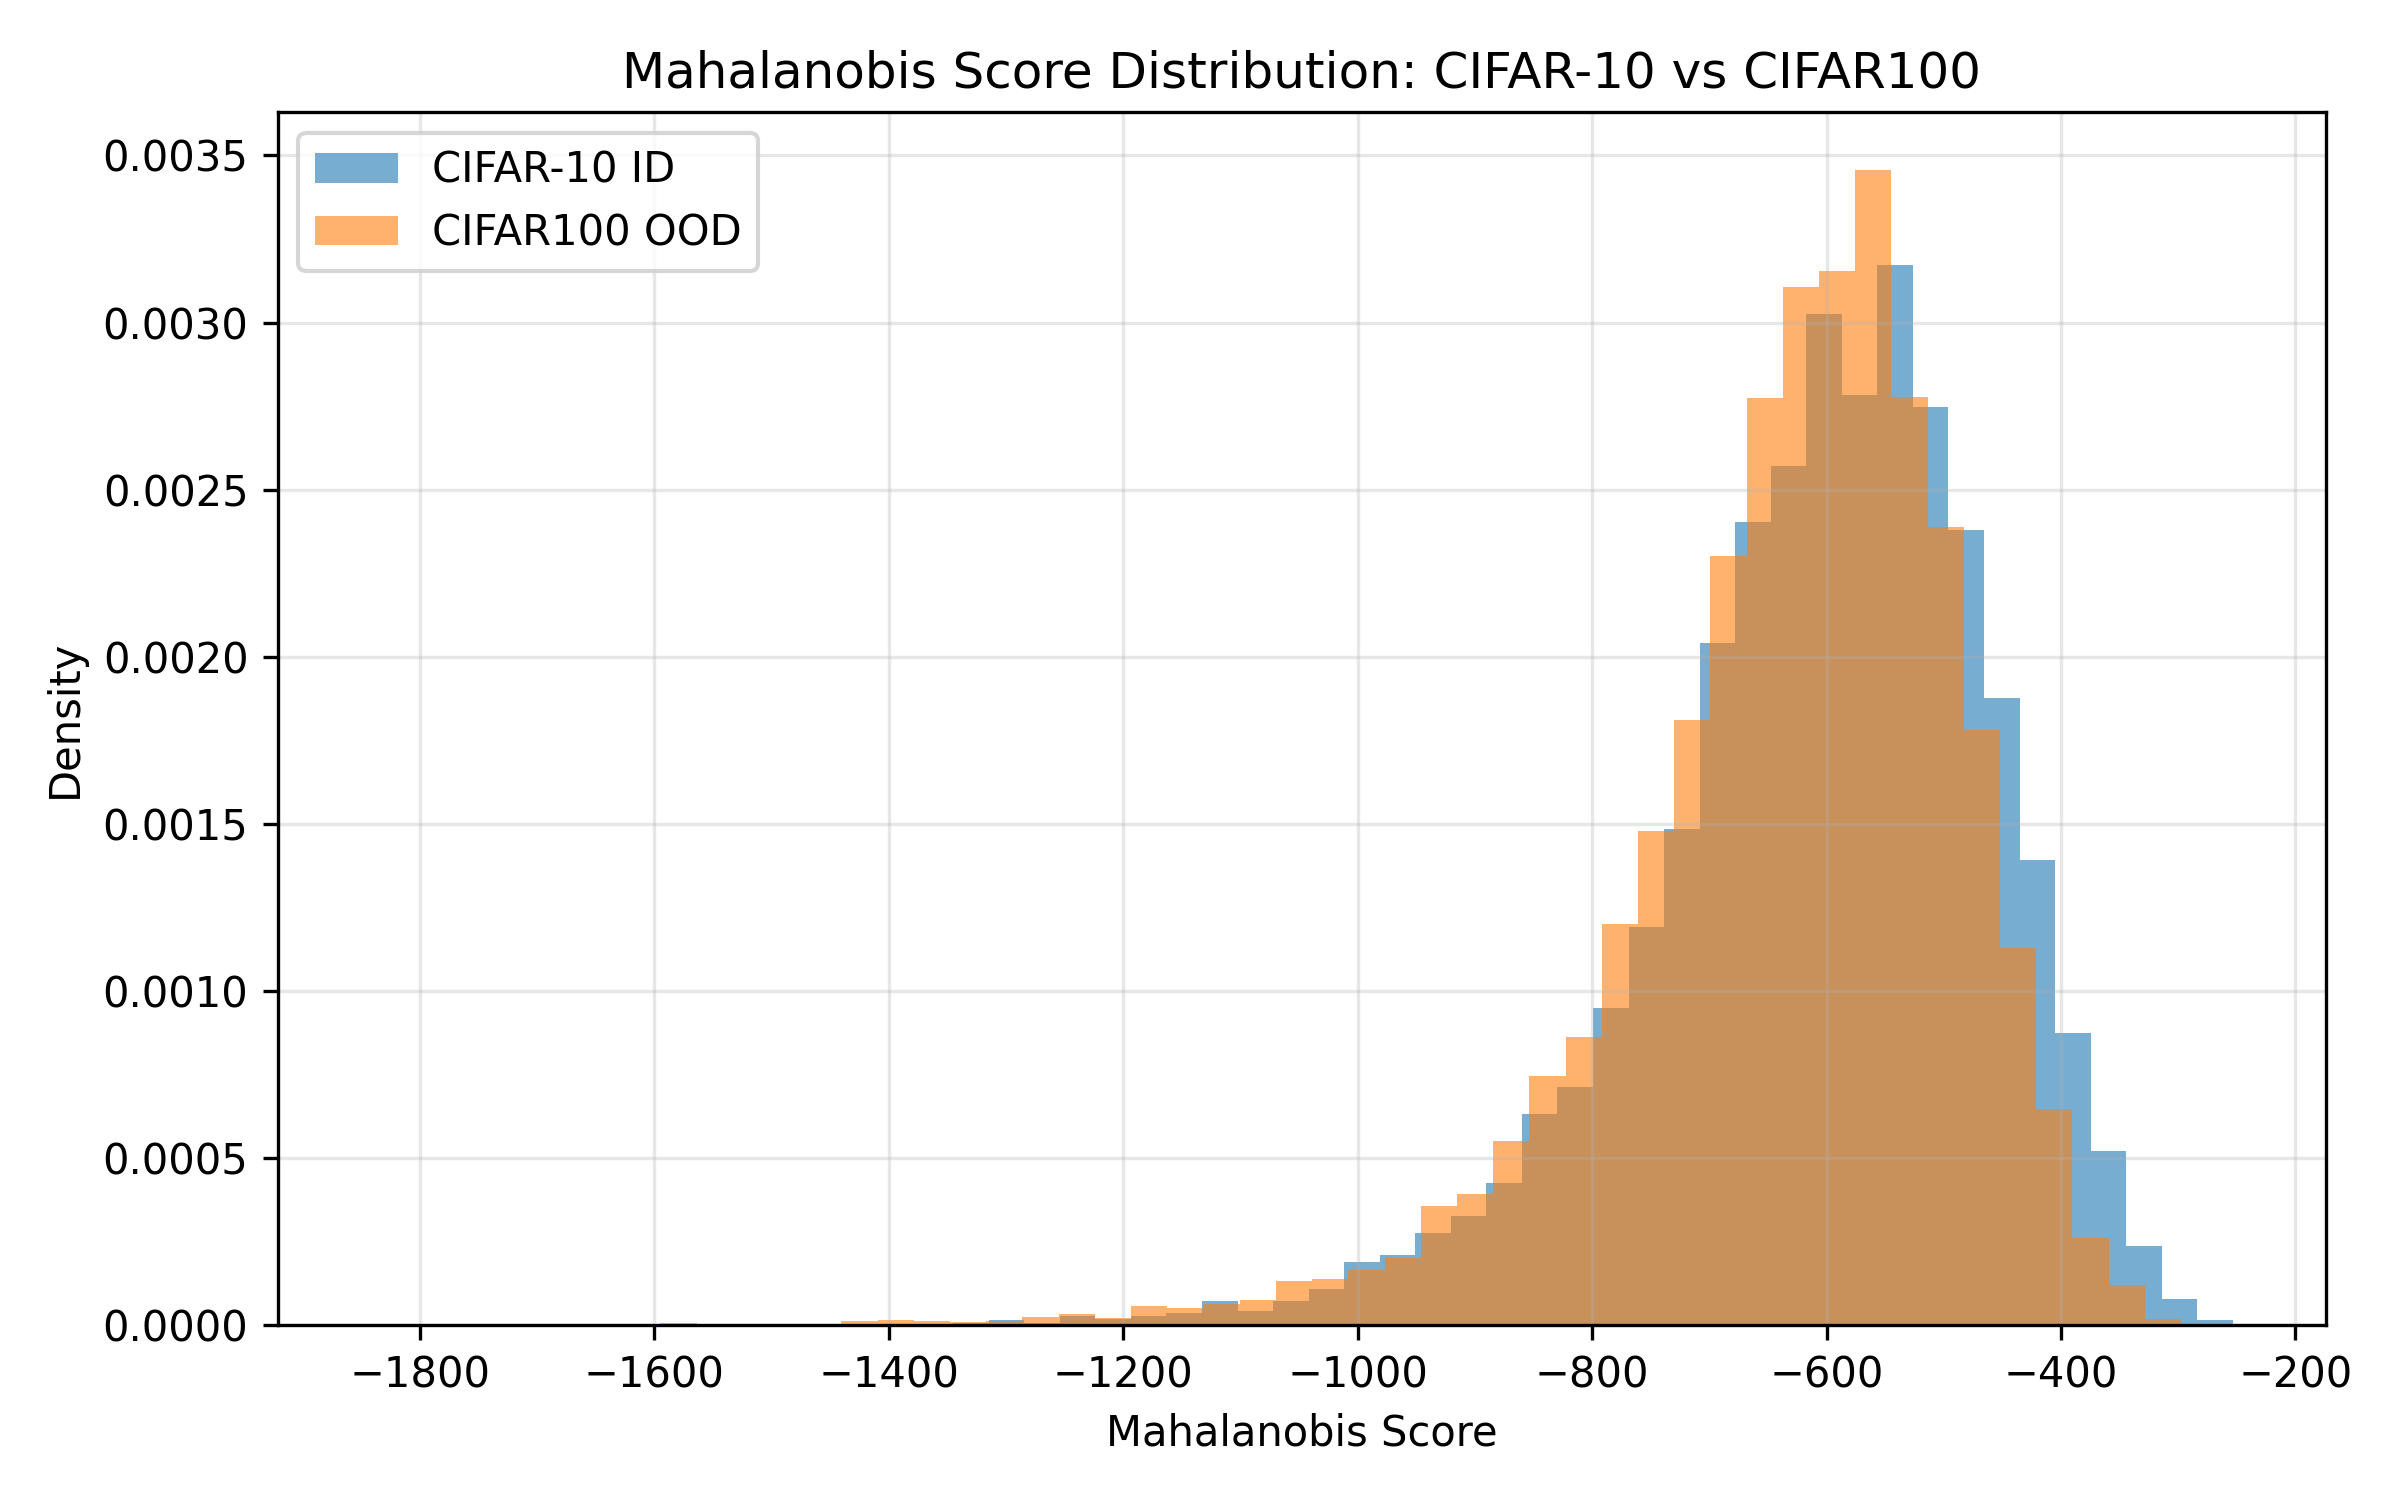
\includegraphics[width=\textwidth]{mahalanobis_cifar10_vs_cifar100.png}
        \caption{Mahalanobis on CIFAR-100.}
    \end{subfigure}
    \caption{Examples of score distributions generated by the project.}
    \label{fig:score-distributions}
\end{figure}

\subsection{ROC Curves}

ROC curves show the trade-off between true positive rate and false positive rate for different thresholds.
The closer the curve is to the top-left corner, the better the separation between ID and OOD samples.

\begin{figure}[H]
    \centering
    \begin{subfigure}{0.32\textwidth}
        \centering
        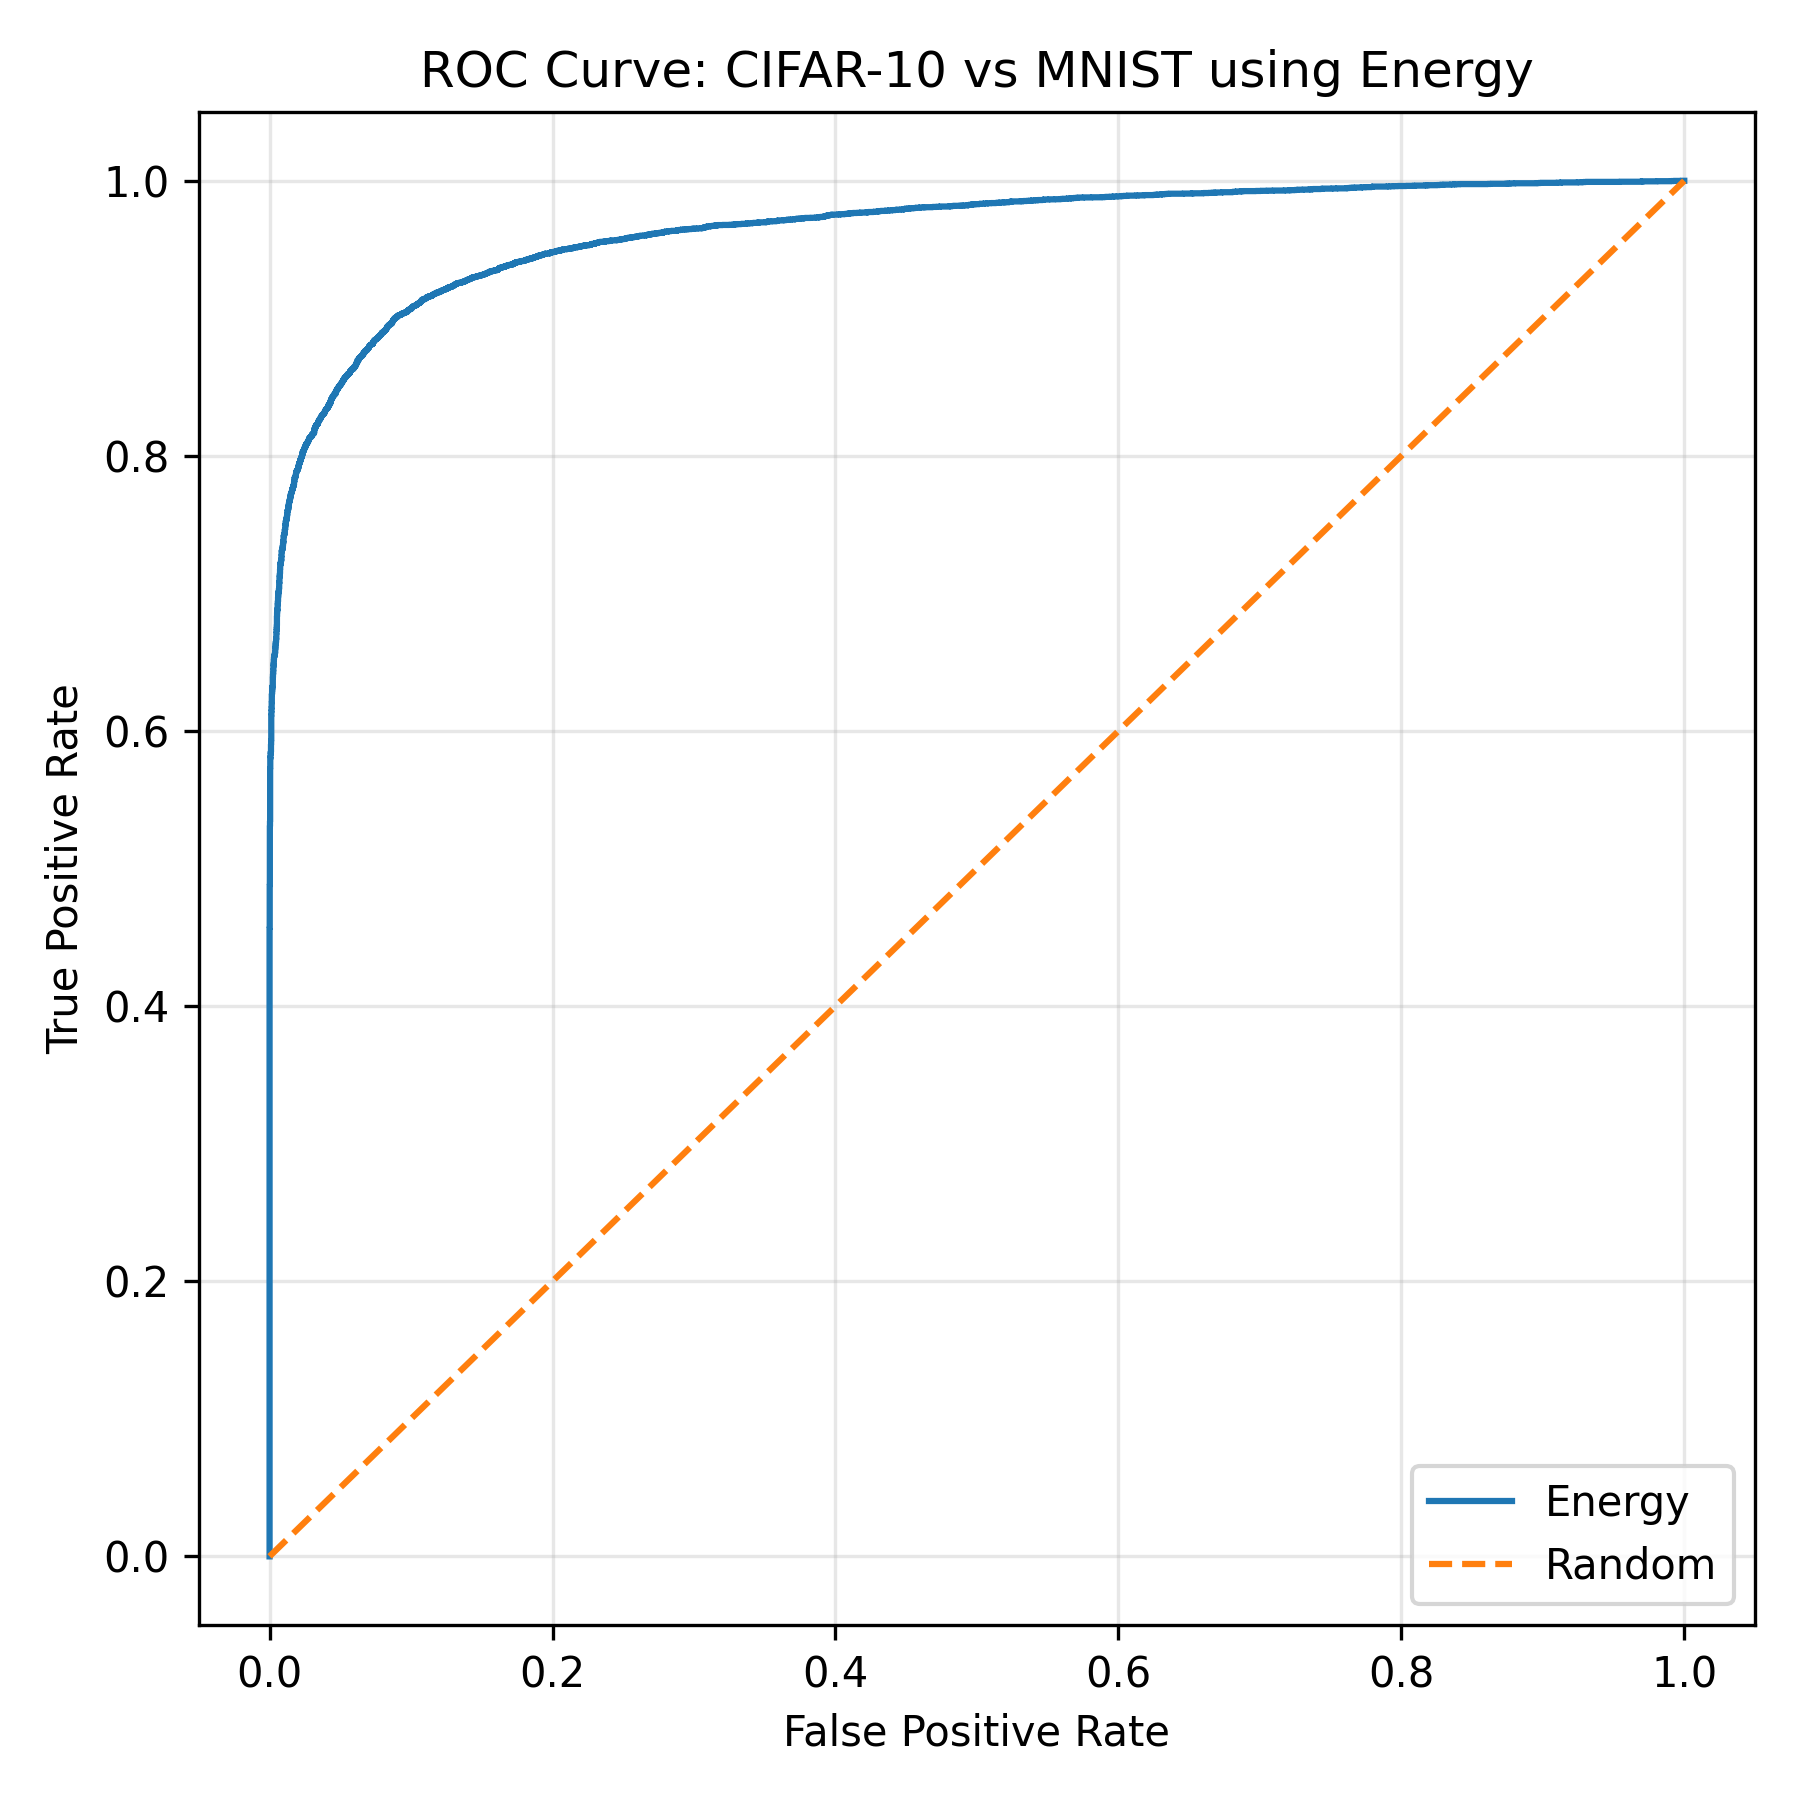
\includegraphics[width=\textwidth]{roc_energy_cifar10_vs_mnist.png}
        \caption{Energy on MNIST.}
    \end{subfigure}
    \hfill
    \begin{subfigure}{0.32\textwidth}
        \centering
        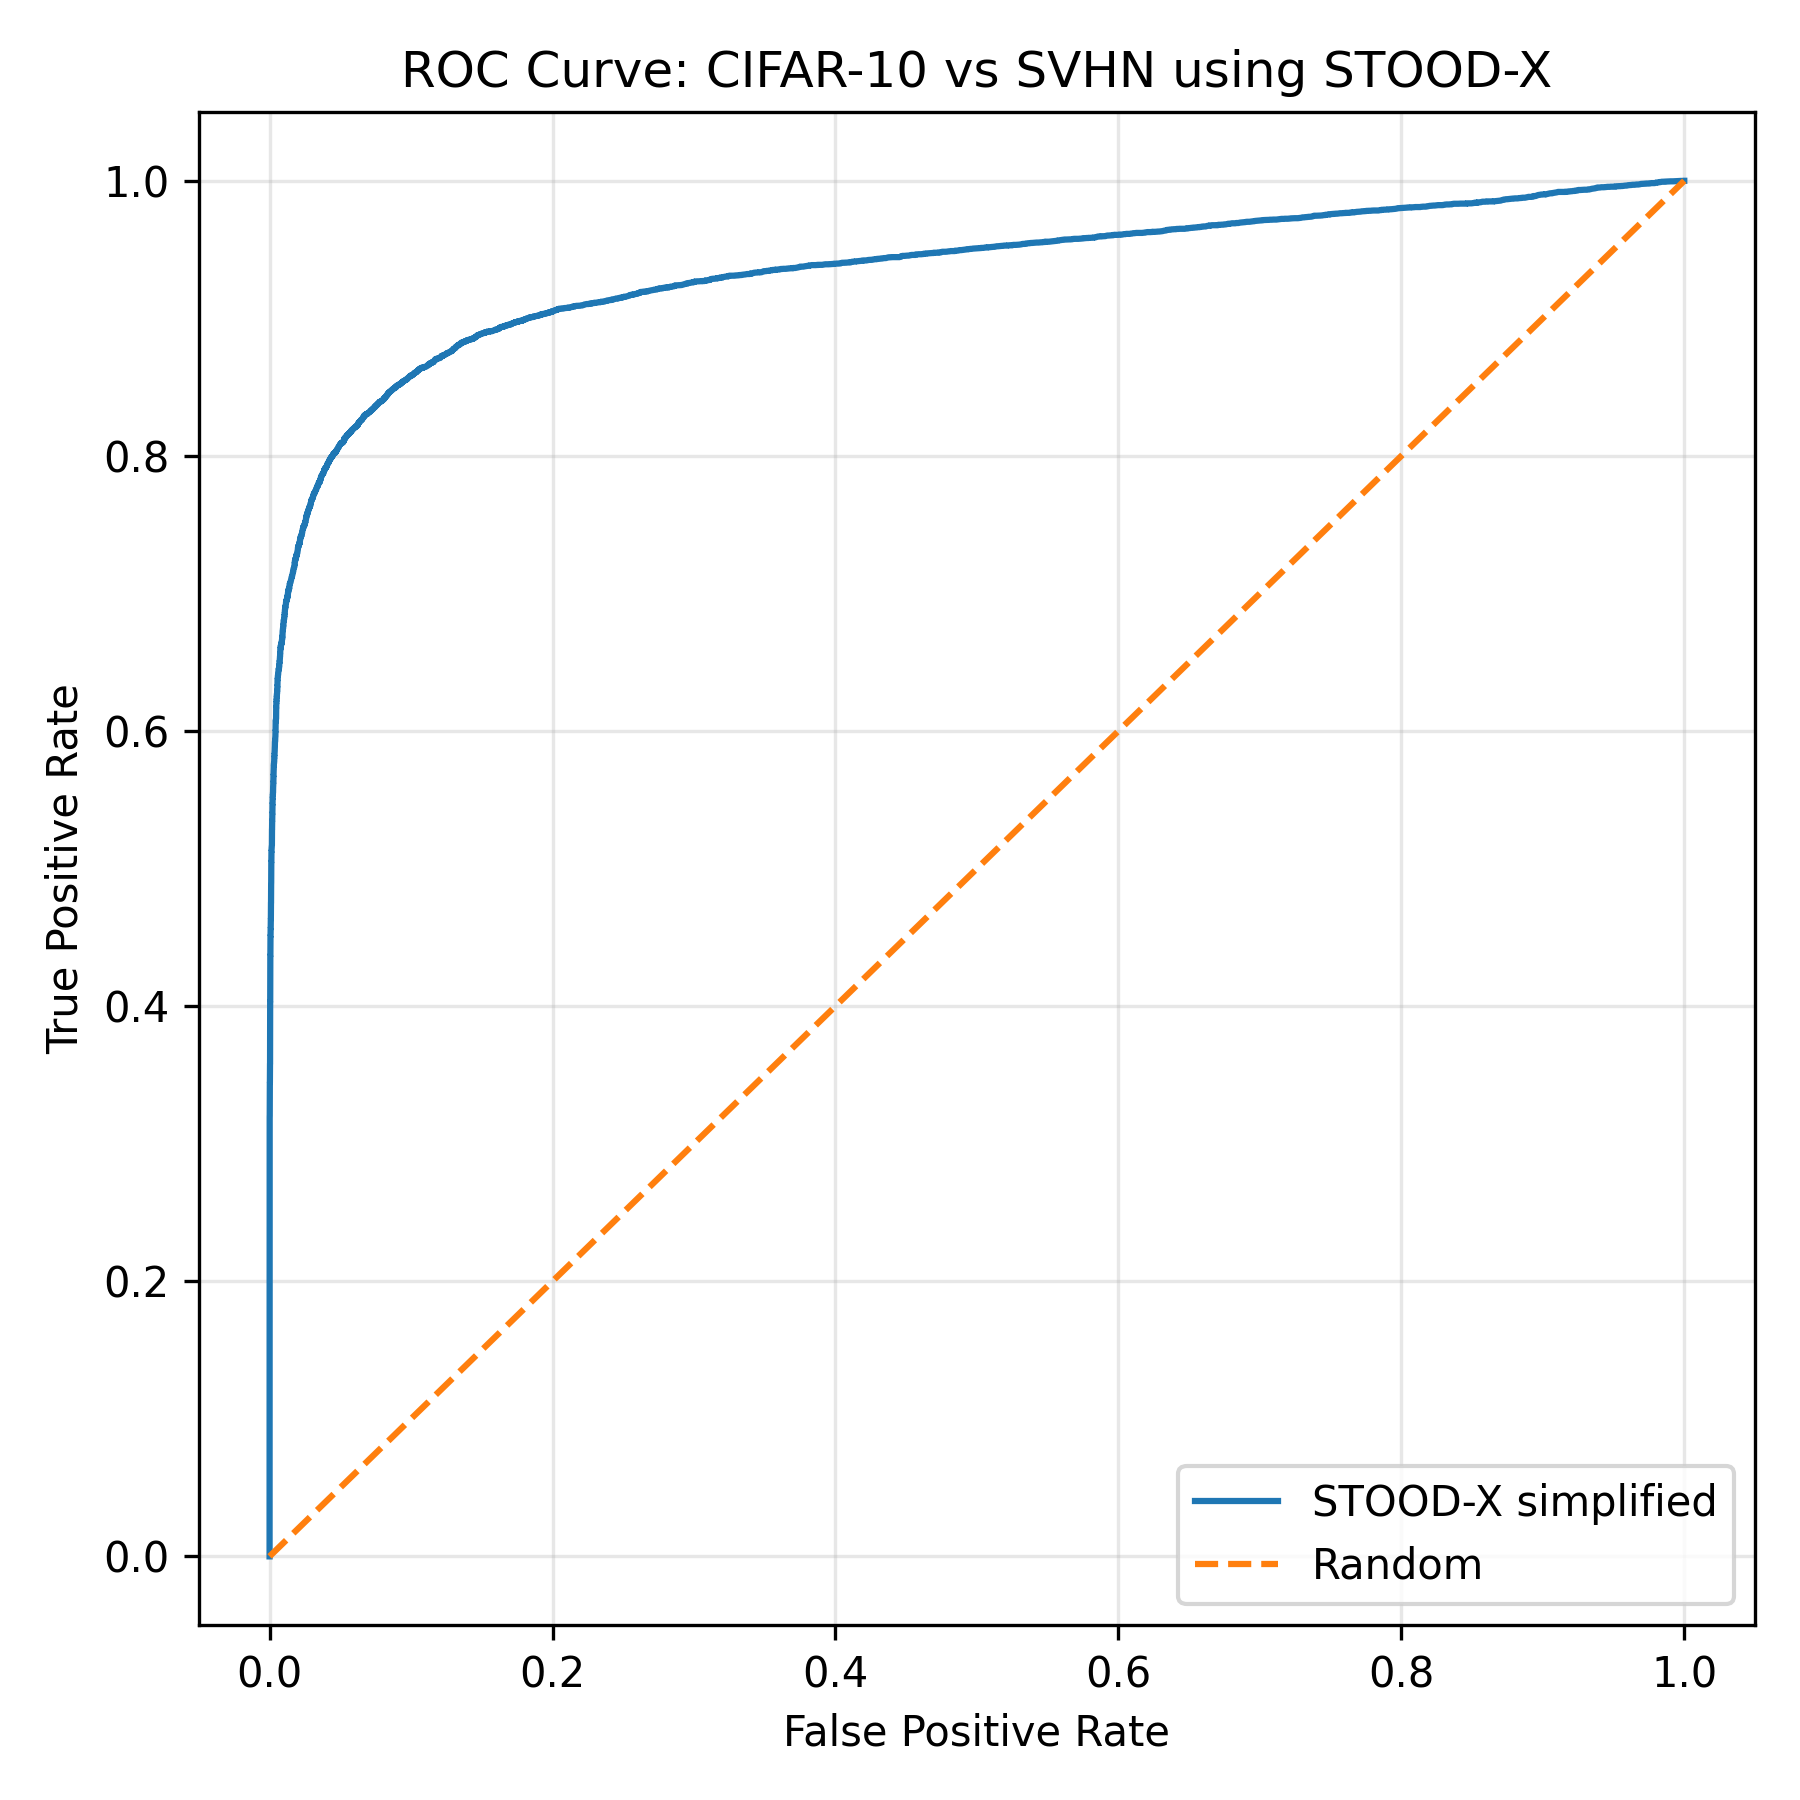
\includegraphics[width=\textwidth]{roc_stoodx_cifar10_vs_svhn.png}
        \caption{STOOD-X on SVHN.}
    \end{subfigure}
    \hfill
    \begin{subfigure}{0.32\textwidth}
        \centering
        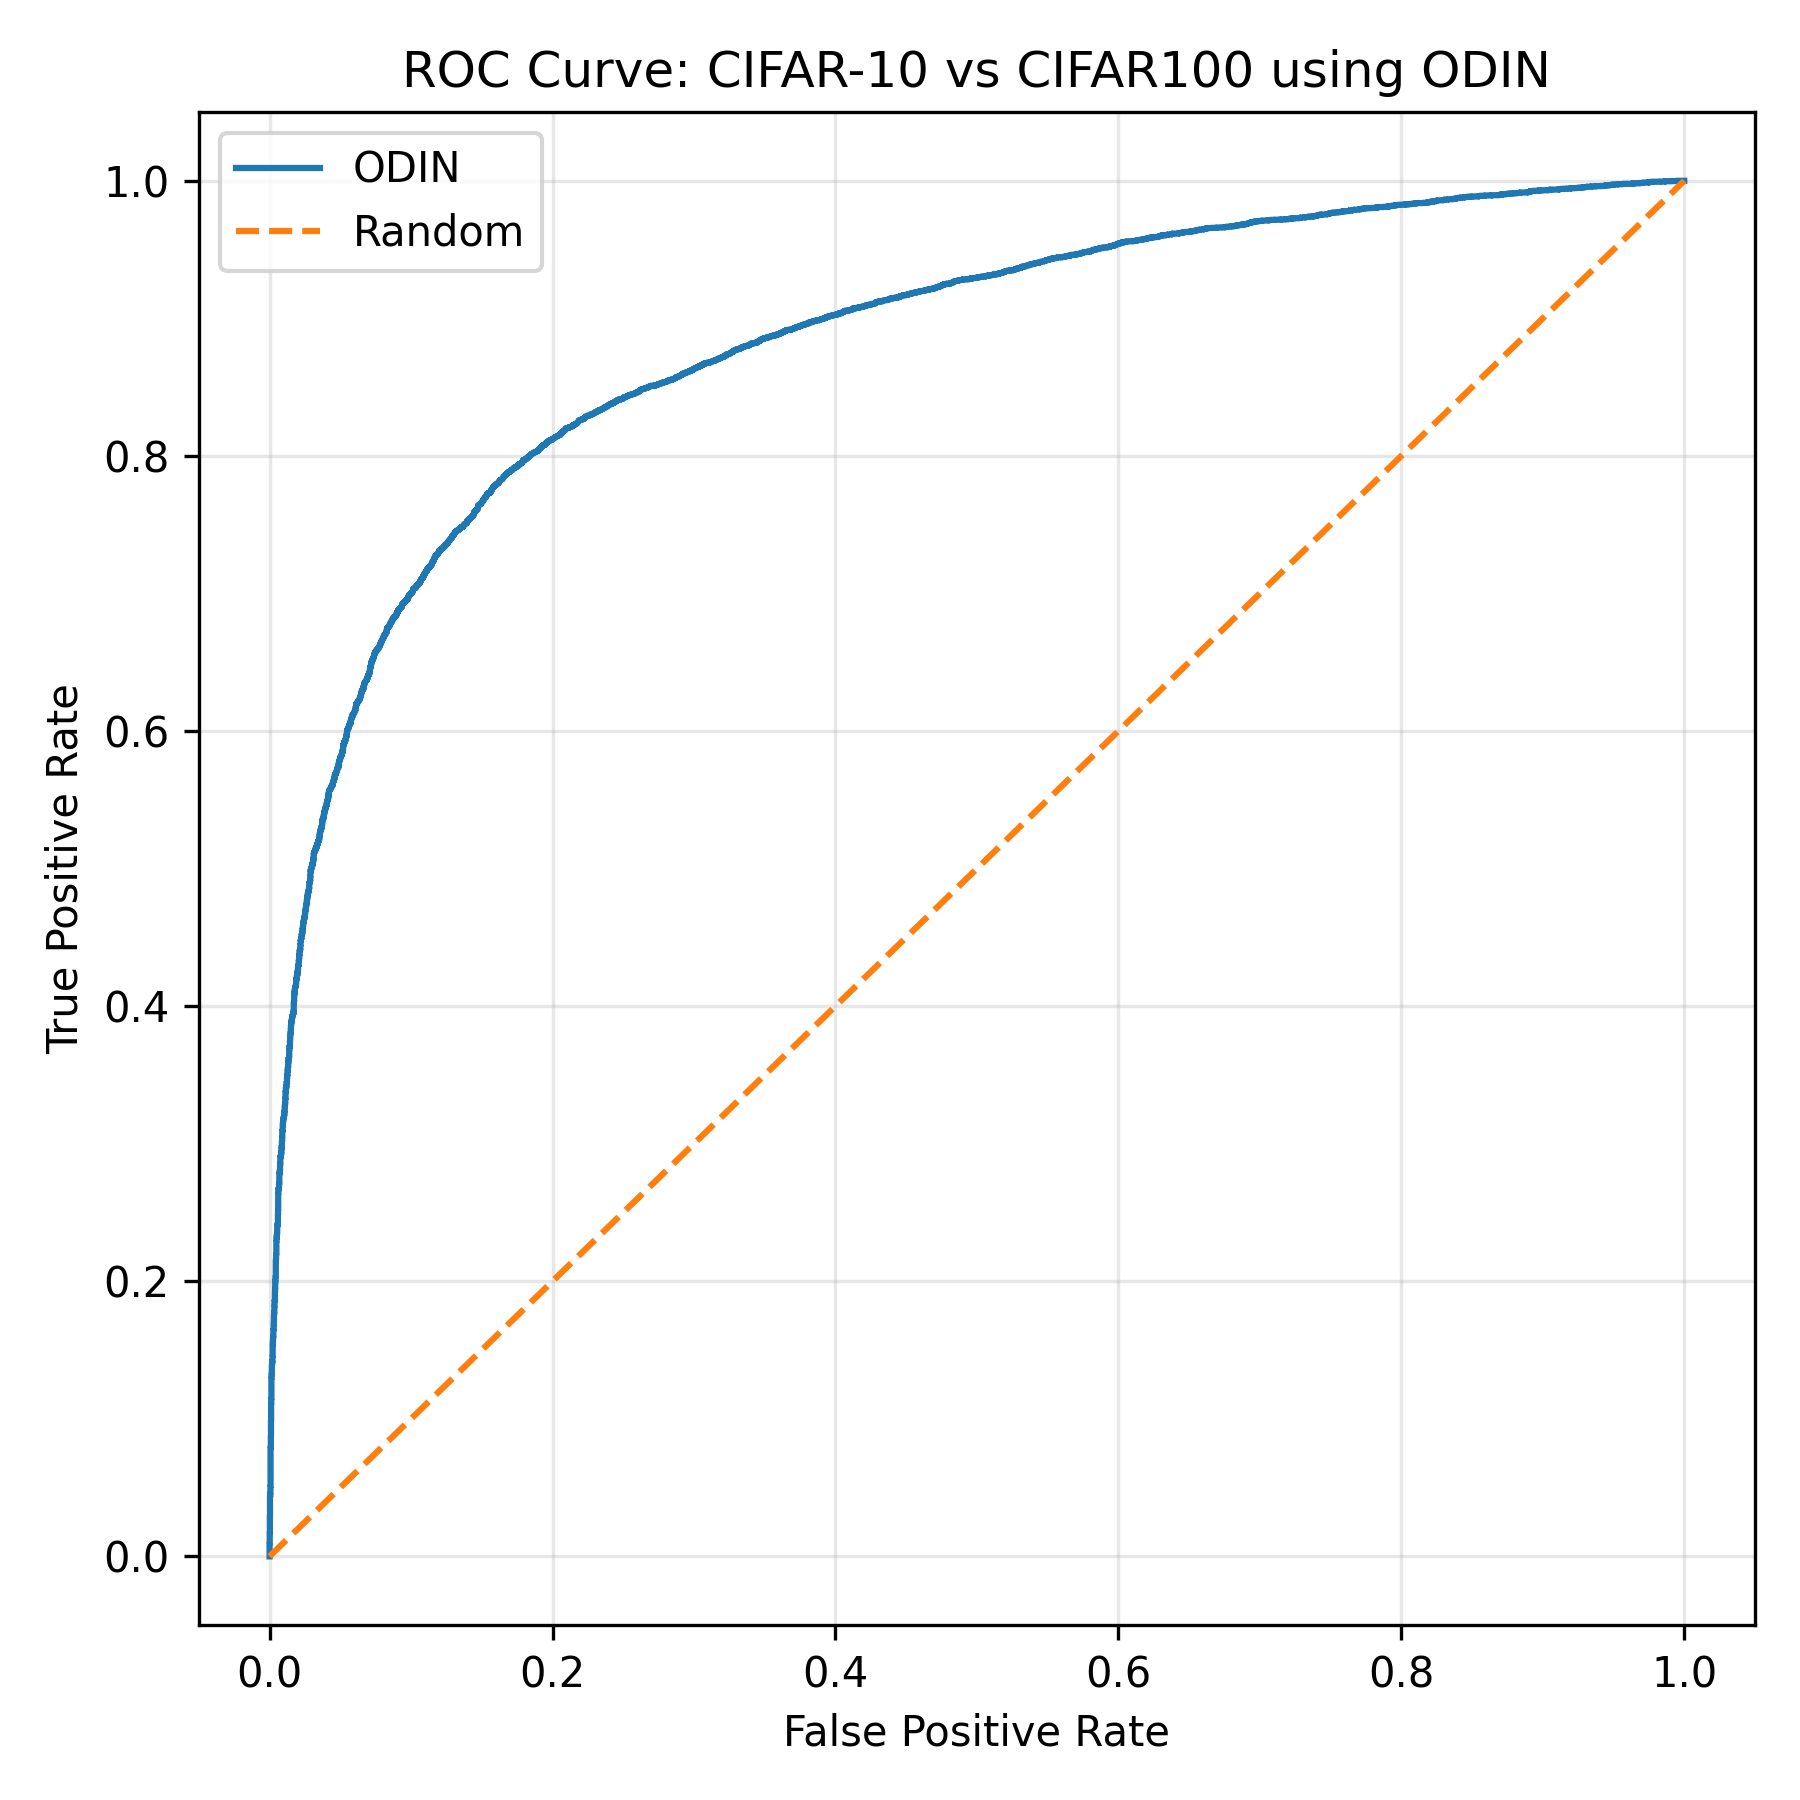
\includegraphics[width=\textwidth]{roc_odin_cifar10_vs_cifar100.png}
        \caption{ODIN on CIFAR-100.}
    \end{subfigure}
    \caption{Examples of ROC curves.}
    \label{fig:roc-curves}
\end{figure}

\subsection{Feature-Space Visualization}

t-SNE and UMAP projections provide a qualitative view of the feature space learned by ResNet-18.
These visualizations help assess whether ID and OOD features form separable regions.
Although they do not replace quantitative metrics, they are useful for interpreting distance-based methods.

\begin{figure}[H]
    \centering
    \begin{subfigure}{0.48\textwidth}
        \centering
        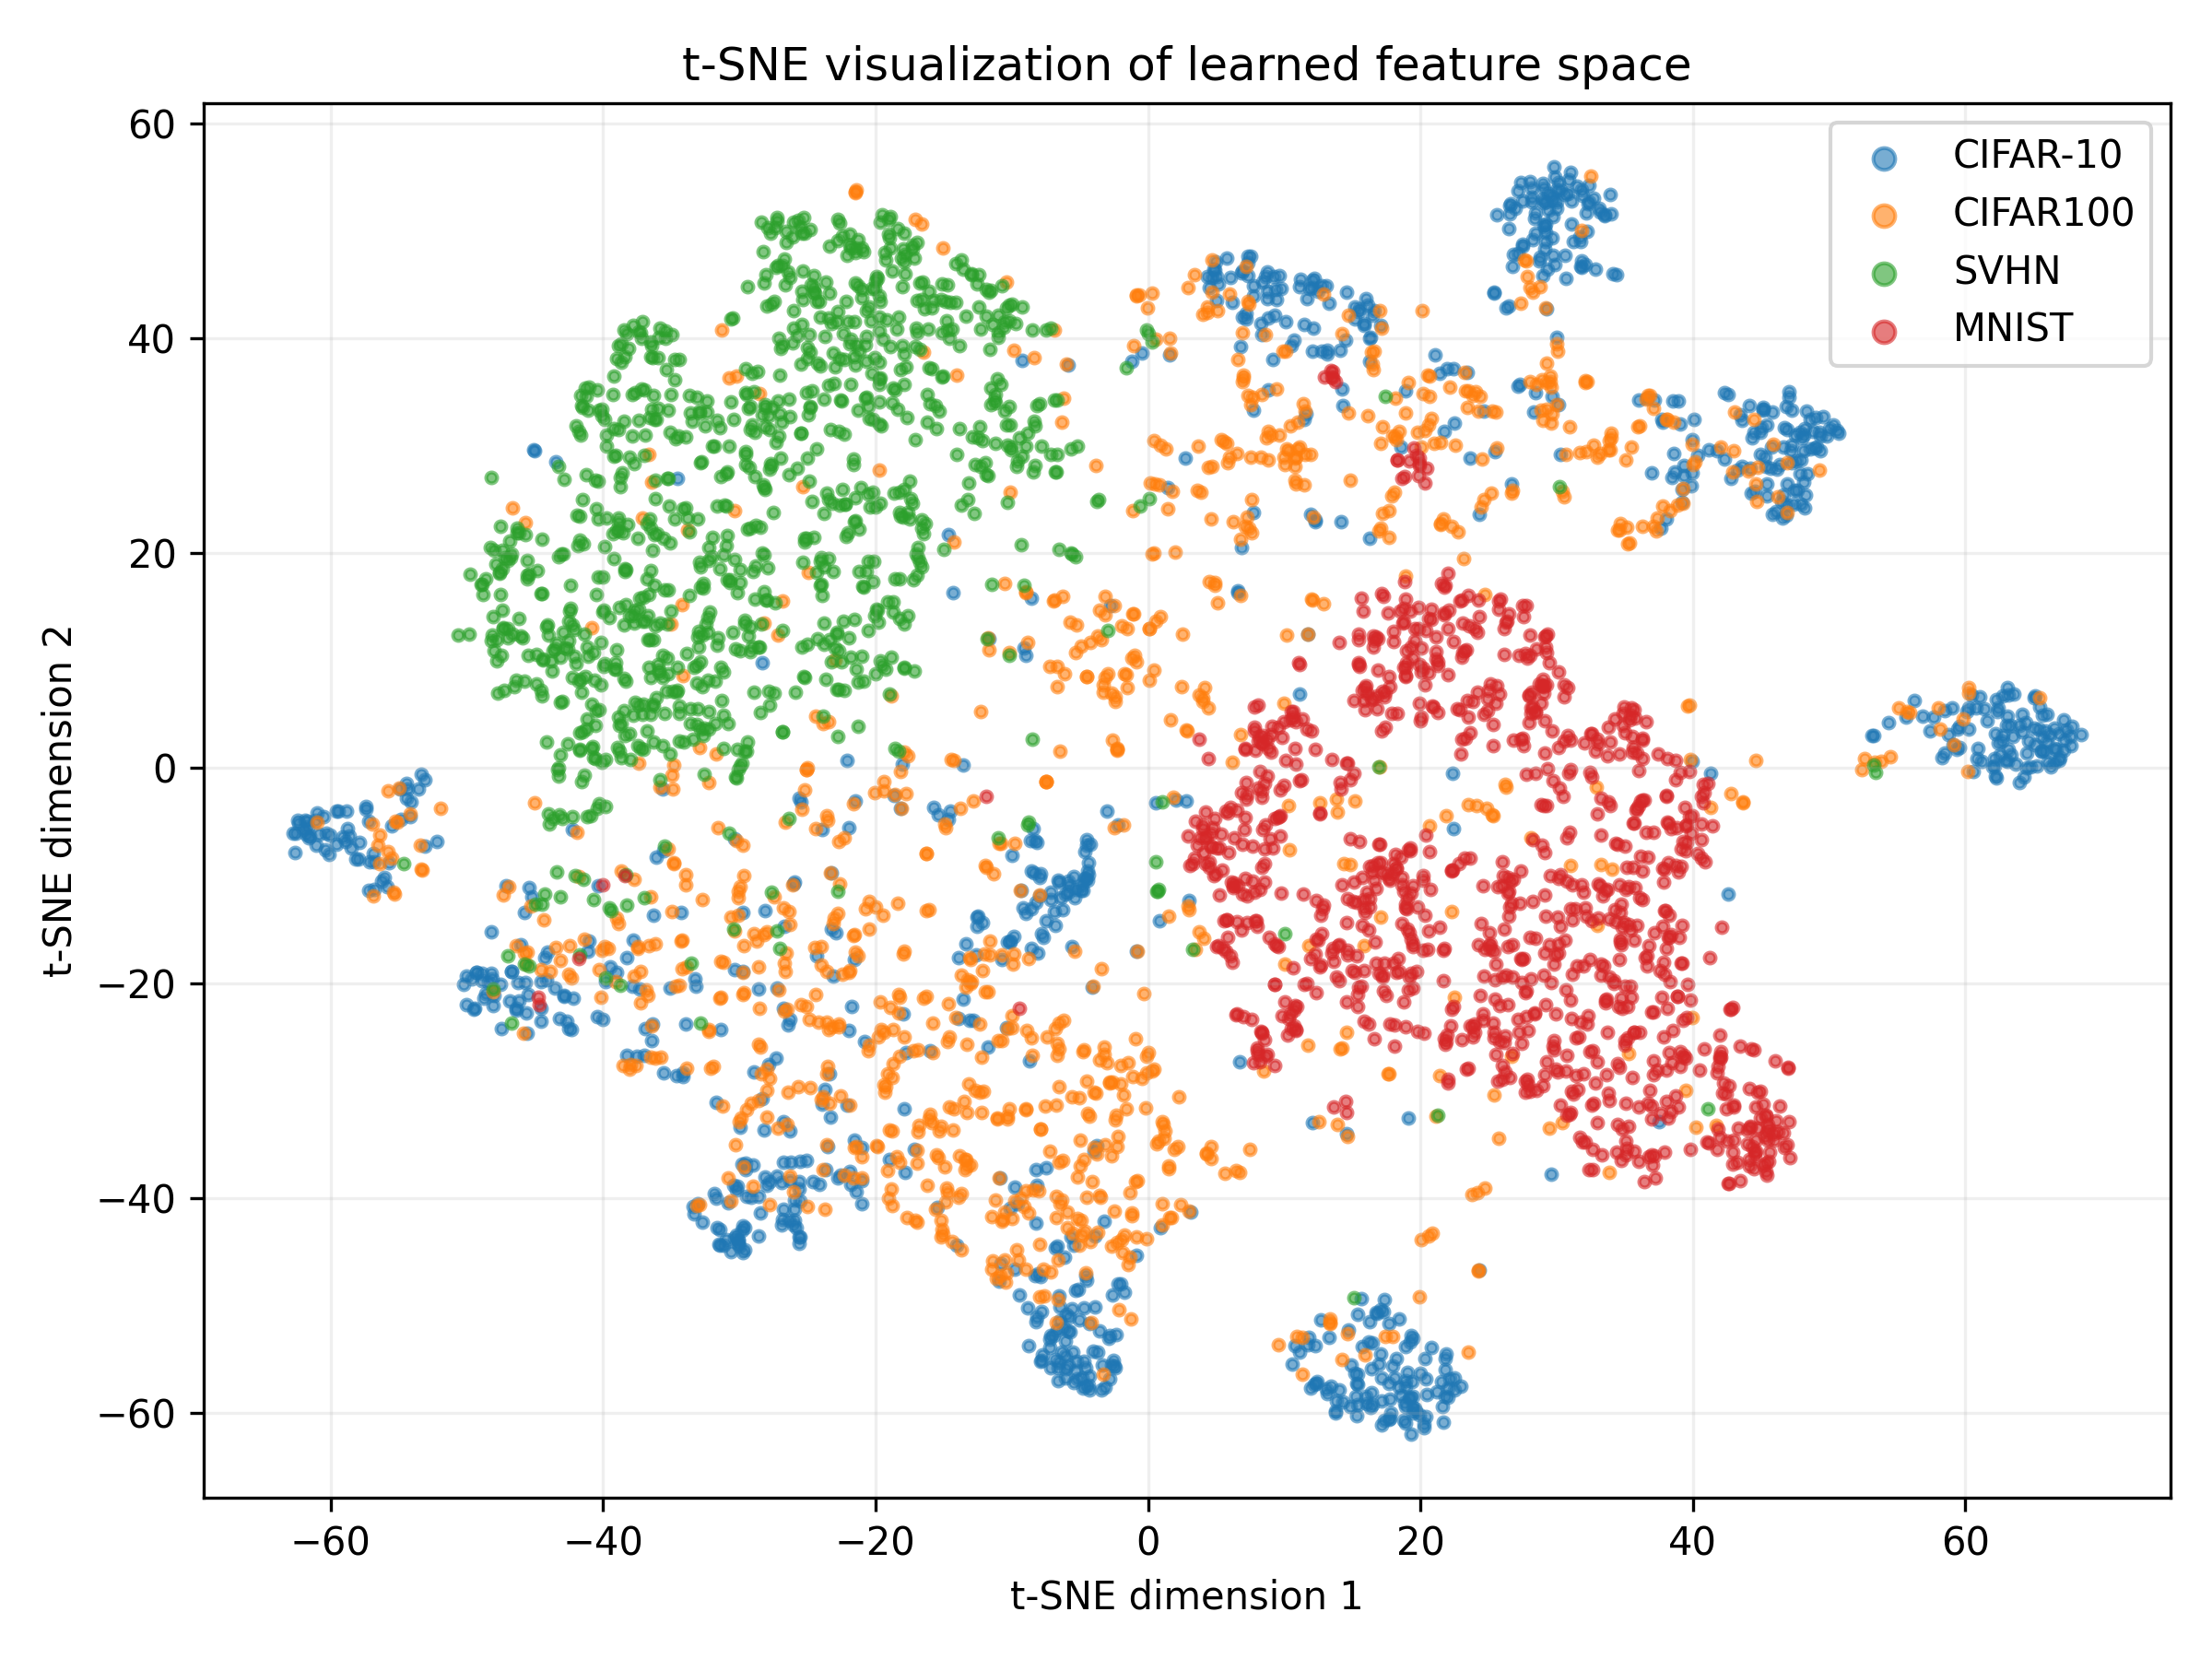
\includegraphics[width=\textwidth]{tsne_cifar10_ood_features.png}
        \caption{t-SNE projection.}
    \end{subfigure}
    \hfill
    \begin{subfigure}{0.48\textwidth}
        \centering
        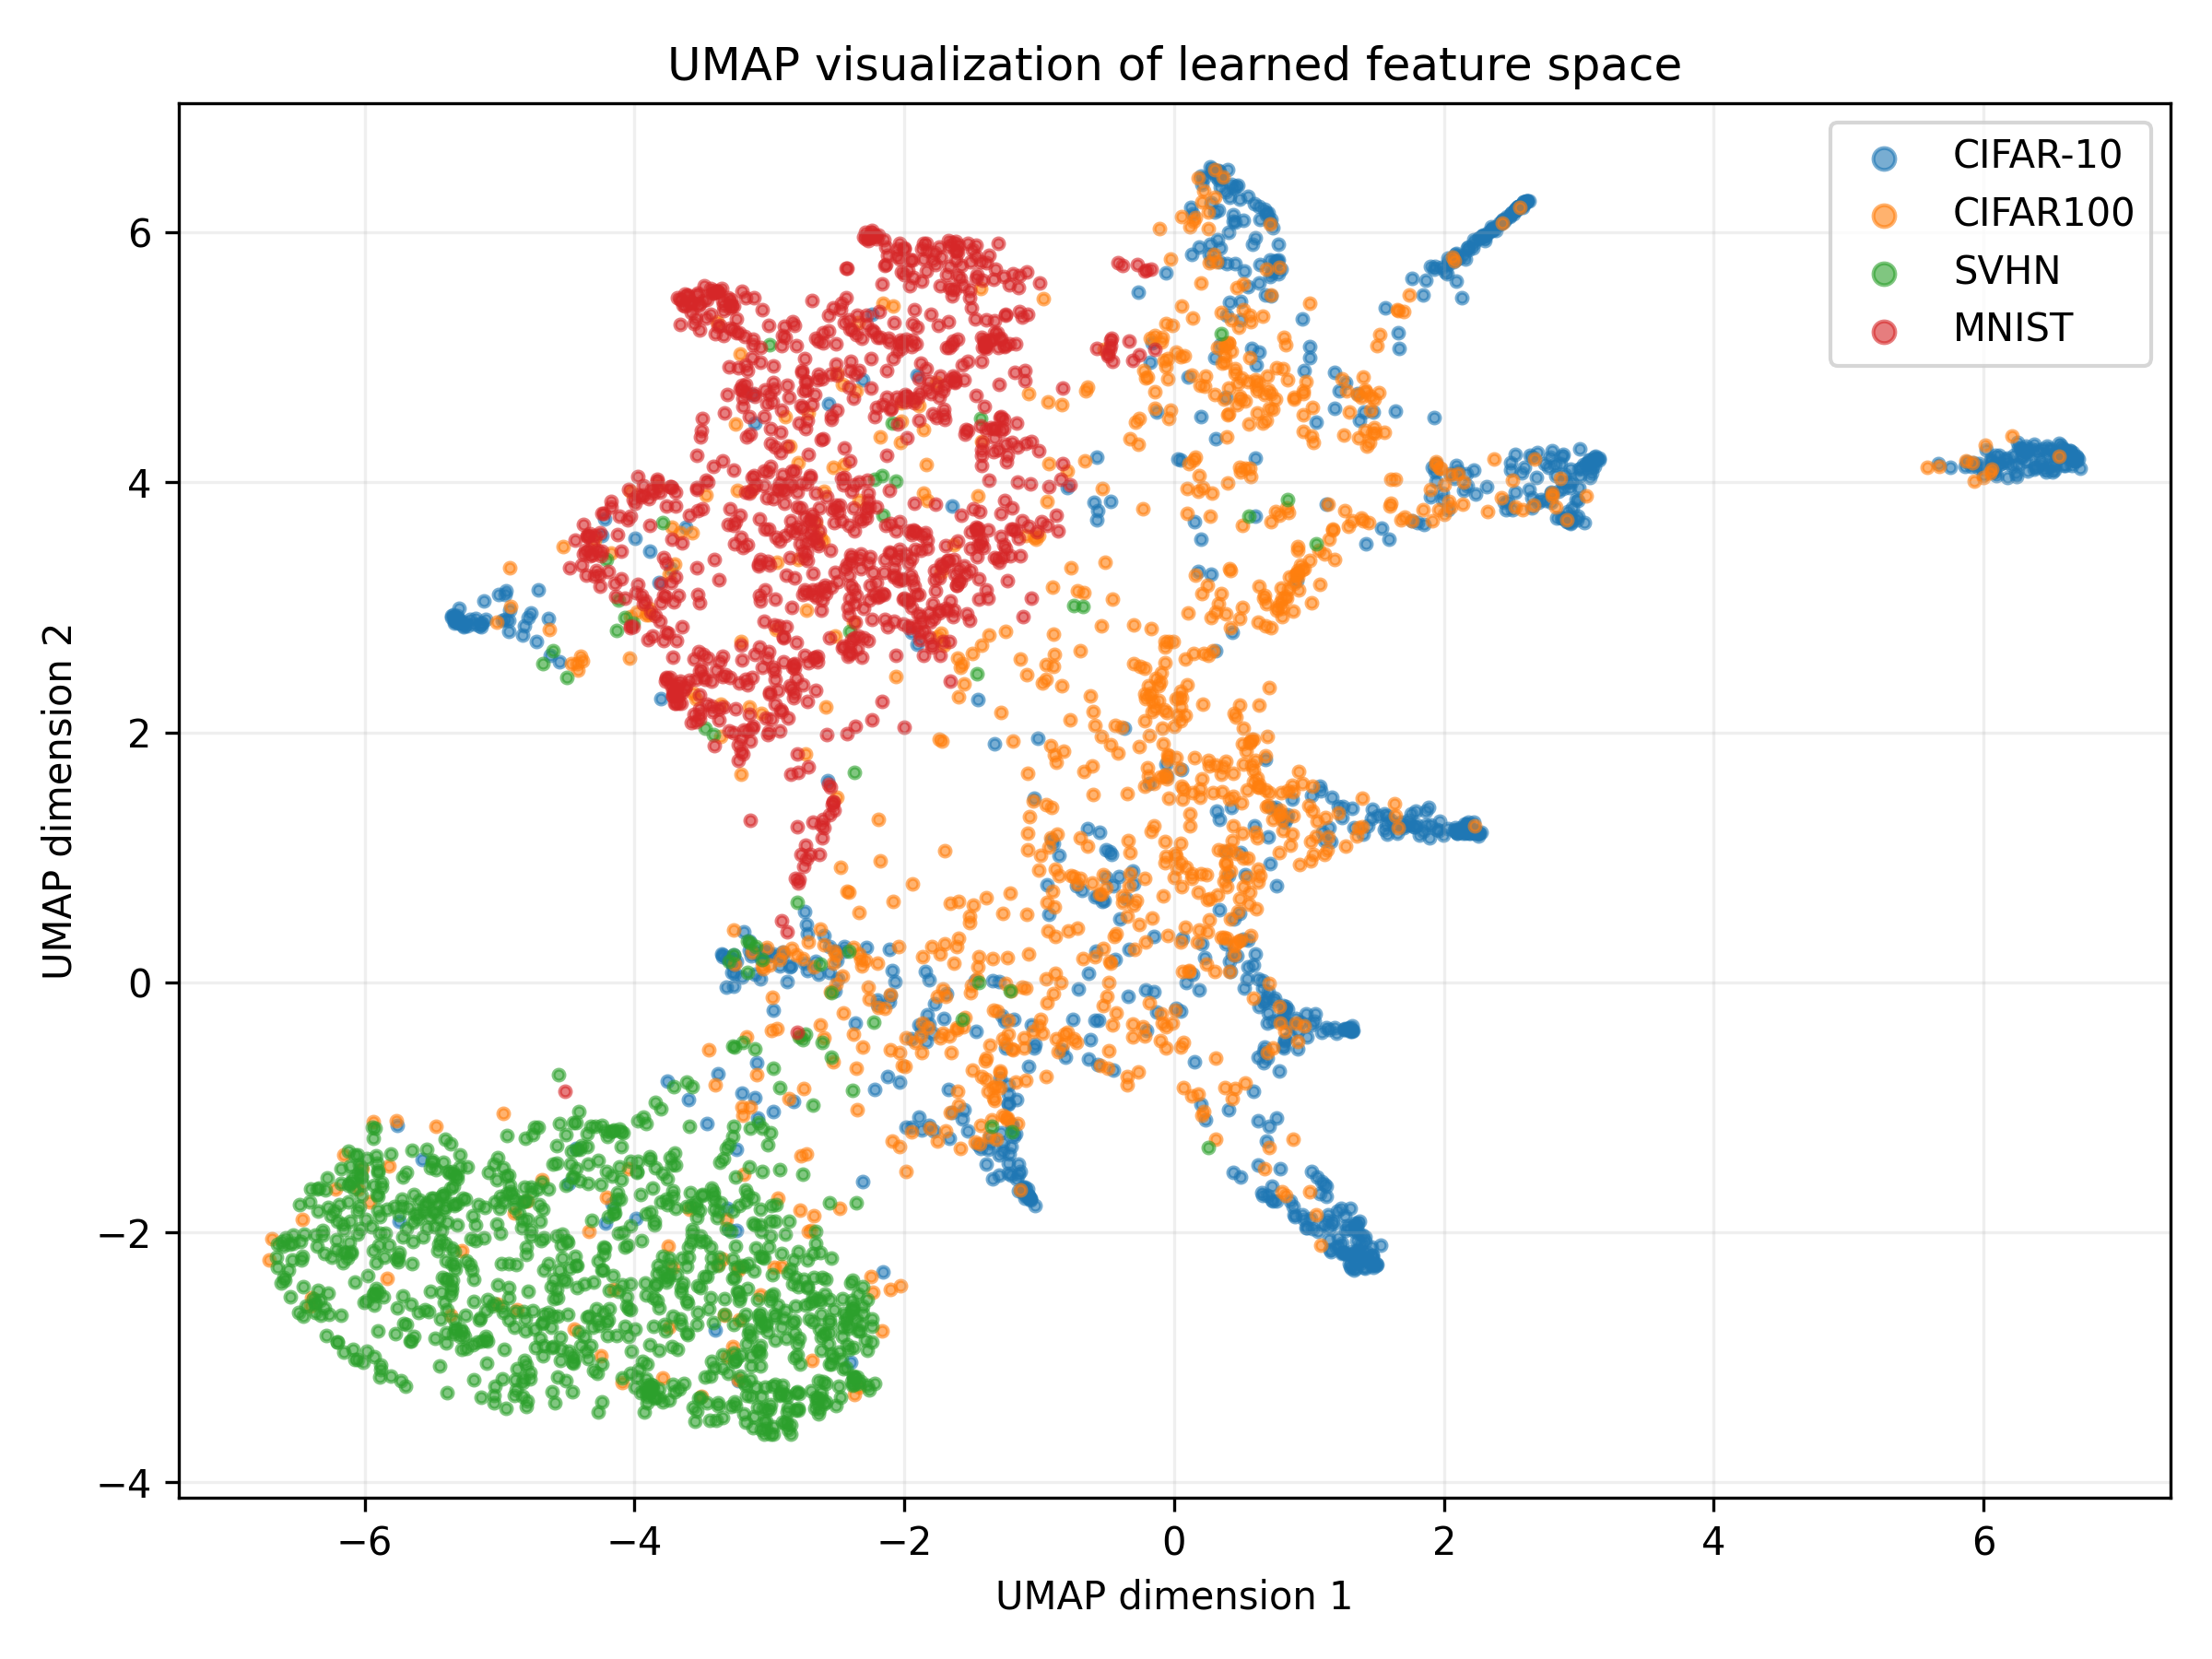
\includegraphics[width=\textwidth]{umap_cifar10_ood_features.png}
        \caption{UMAP projection.}
    \end{subfigure}
    \caption{Two-dimensional projections of CIFAR-10 and OOD features.}
    \label{fig:tsne-umap}
\end{figure}

\subsection{Confusion Matrix}

The confusion matrix shows the behavior of the base classifier on CIFAR-10.
This step is important because OOD detection methods depend on the quality of the features and logits produced by this classifier.

\begin{figure}[H]
    \centering
    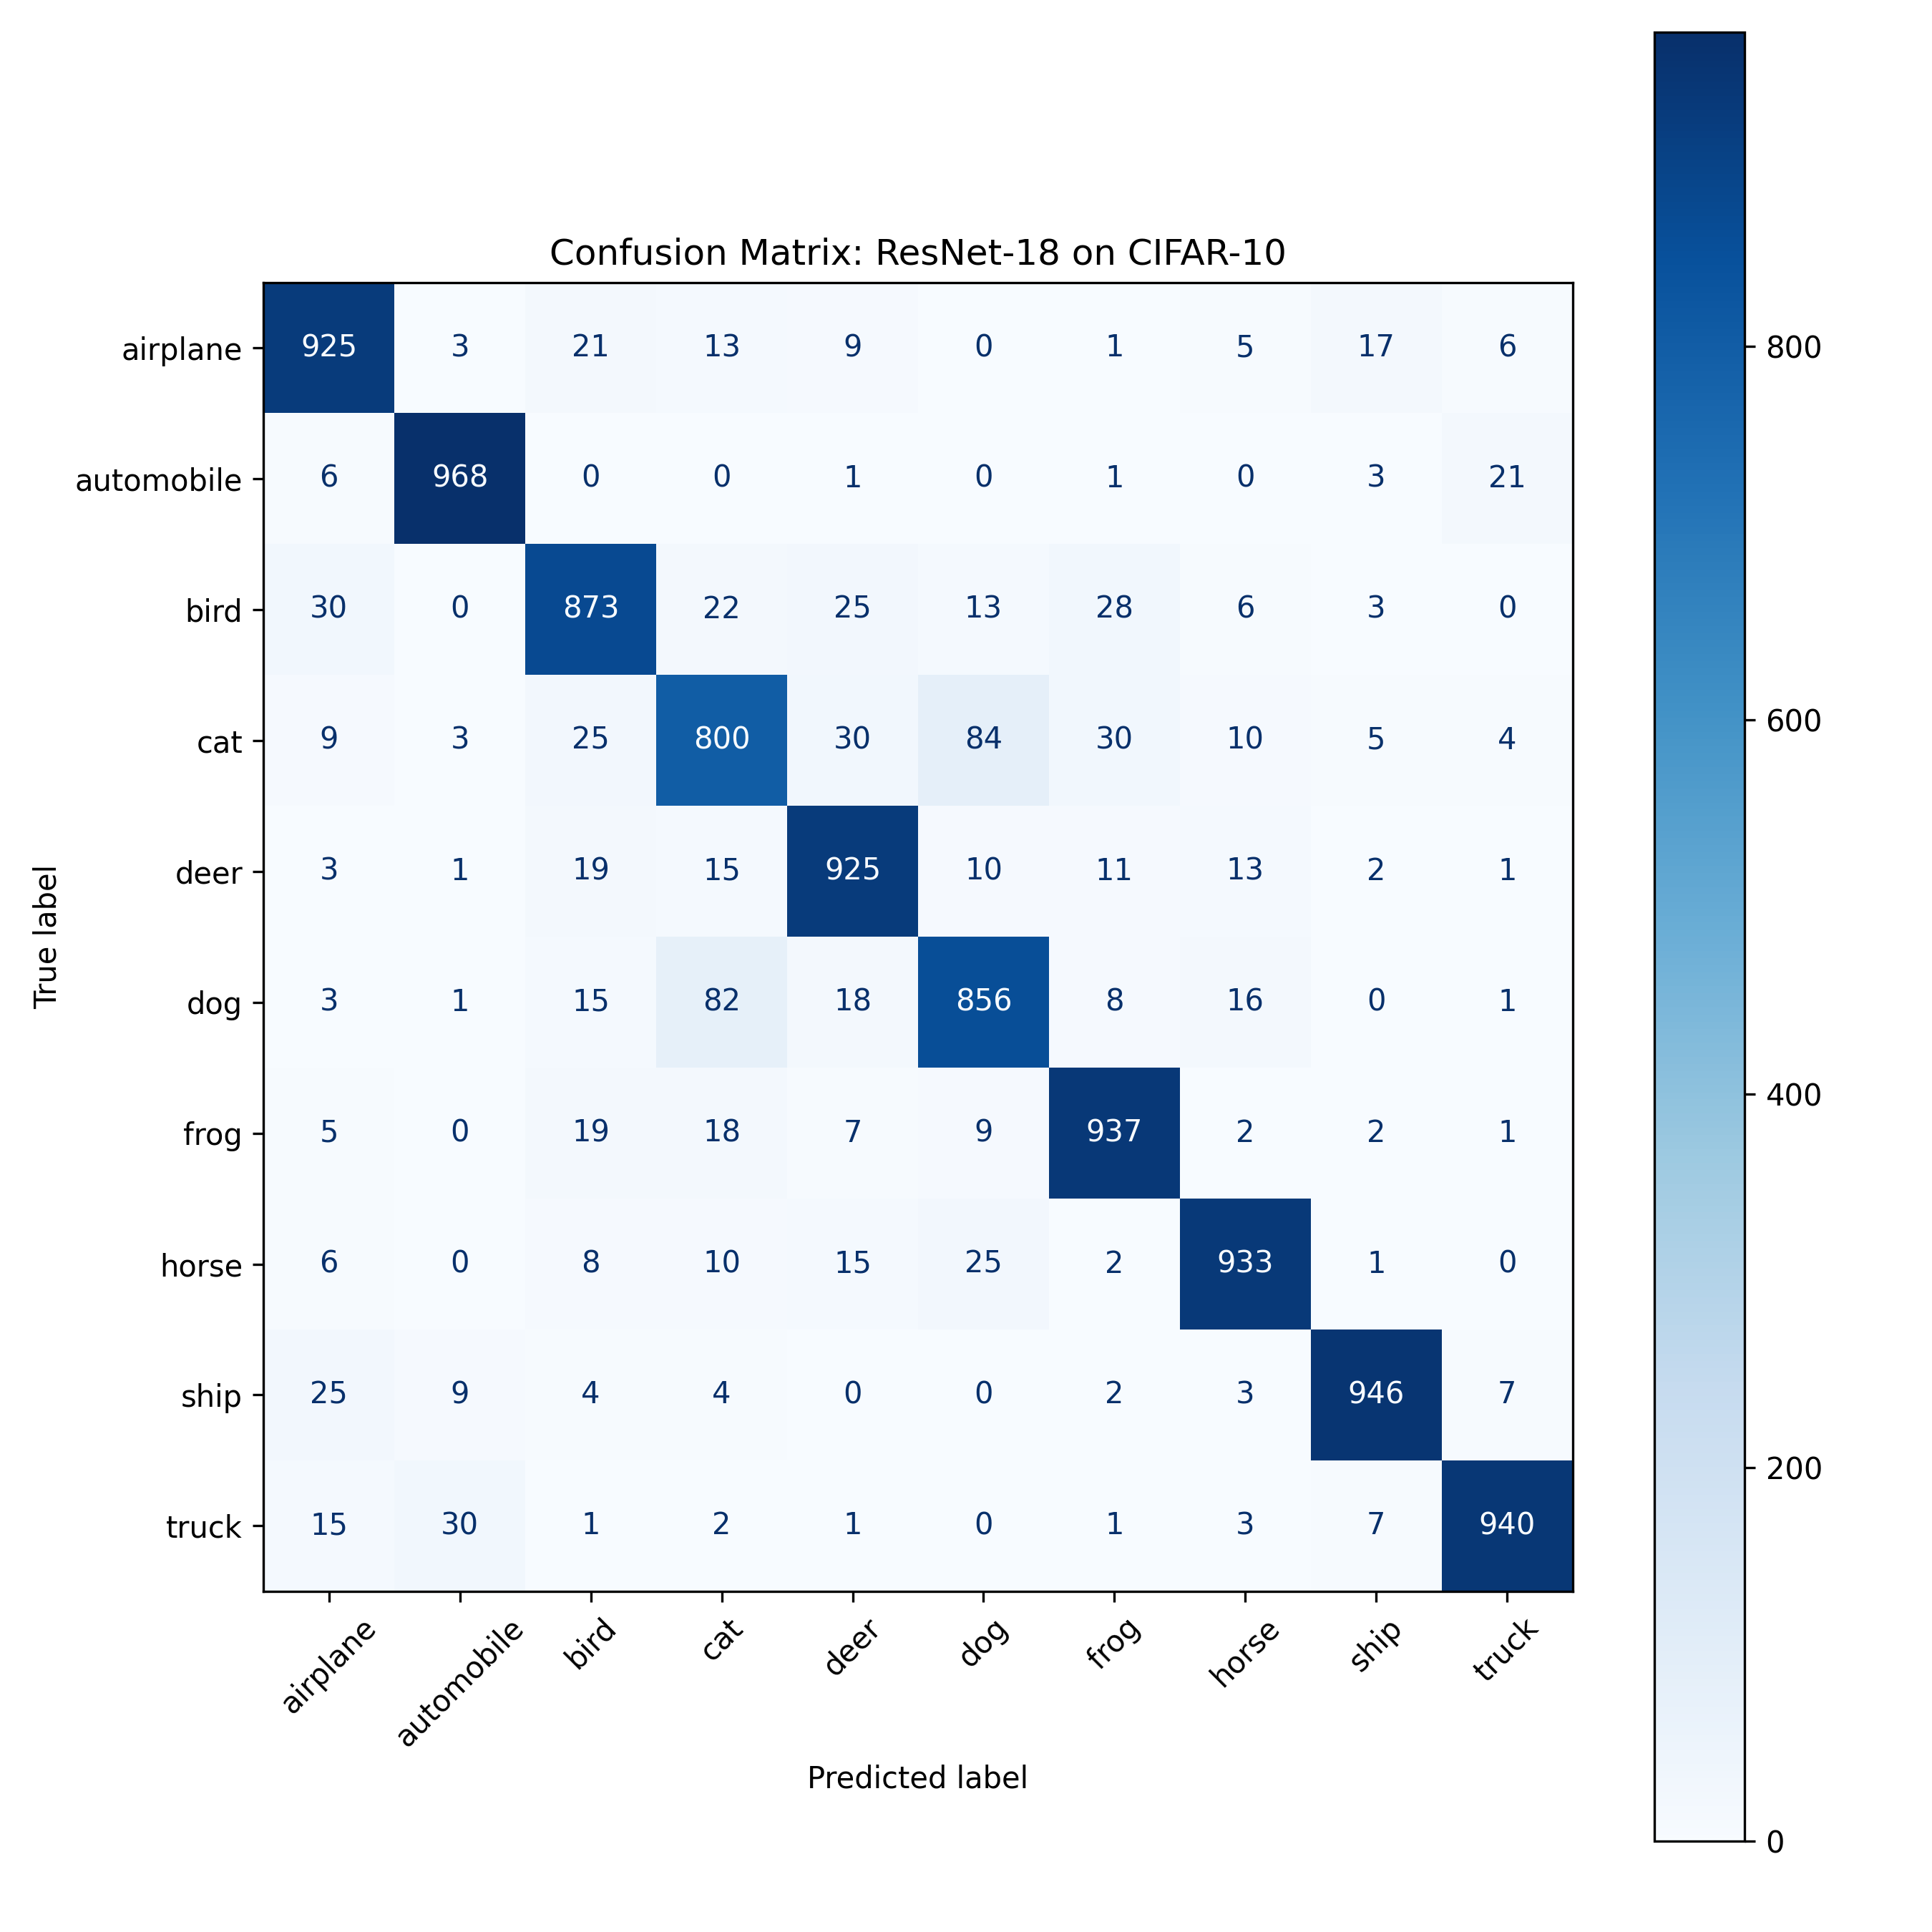
\includegraphics[width=0.72\textwidth]{confusion_matrix_resnet18_cifar10.png}
    \caption{Confusion matrix of ResNet-18 on CIFAR-10.}
    \label{fig:confusion-matrix}
\end{figure}

\section{Discussion}

The results show that different methods capture different signals.
MSP is simple and fast, but it suffers from neural network overconfidence.
Energy and ODIN improve this baseline because they make better use of the logit structure.
For this reason, they show very strong performance on CIFAR-100 and MNIST.

KNN and the simplified STOOD-X method depend on the geometry of the feature space.
On SVHN, these methods outperform Energy and ODIN.
This indicates that, although the classifier may still produce relatively confident logits, SVHN features are farther away from the typical neighborhood structure of CIFAR-10 features.

The Mahalanobis method performs poorly in this experiment.
One likely cause is the simplified implementation, which uses only the penultimate layer, a single global covariance matrix and limited regularization.
In addition, the assumption that the features are approximately Gaussian may not be appropriate.

The simplified STOOD-X method performs very similarly to KNN, which is expected.
Both methods start from the same KNN distance.
The difference is that STOOD-X converts the distance into an empirical p-value, which provides a statistical interpretation: high scores indicate greater compatibility with the ID reference distribution.

\section{Limitations}

The project has several limitations:

\begin{itemize}
    \item the replication of the STOOD-X paper is partial, not complete;
    \item the STOOD-X implementation is simplified and does not fully reproduce the Wilcoxon-Mann-Whitney test described in the original paper;
    \item the visual explainability stage of STOOD-X was not implemented;
    \item the datasets, architectures and experimental protocols are smaller in scope than those used in the paper;
    \item the results were obtained from a single run, without multiple random seeds;
    \item the method hyperparameters were not extensively optimized;
    \item Mahalanobis uses only penultimate-layer features;
\end{itemize}

\section{Future Work}

As future work, it would be relevant to:

\begin{itemize}
    \item implement the original STOOD-X method with the Wilcoxon-Mann-Whitney test;
    \item add the concept-based visual explainability stage;
    \item repeat the experiments with several random seeds and report mean and standard deviation;
    \item test additional OOD datasets and stronger architectures;
    \item compare with additional methods such as ReAct, ViM, ASH or RMDS;
    \item improve Mahalanobis with multi-layer features and covariance calibration;
\end{itemize}

\section{Conclusion}

This project presents a partial and adapted replication of the STOOD-X paper, framed as a comparative study of OOD detection methods in computer vision.
Instead of fully reproducing the original methodology, the work focuses on its central idea: using the feature space of a trained network to evaluate whether a new sample is compatible with the known distribution.

For this purpose, a ResNet-18 model trained on CIFAR-10 was used.
The results show that there is no single method that is universally best across all scenarios.
Energy and ODIN are the strongest methods on CIFAR-100 and MNIST, while KNN and the simplified STOOD-X method perform best on SVHN.

The simplified STOOD-X implementation shows that feature-space distances can be transformed into scores with a statistical interpretation.
However, this implementation still does not correspond to the full STOOD-X method described in the original paper, mainly because it does not include the Wilcoxon-Mann-Whitney test or the visual explainability component.
Even so, the project provides a useful experimental basis for studying OOD detection and for developing a more complete, robust and explainable version in the future.

\begin{thebibliography}{9}

\bibitem{hendrycks2017}
Dan Hendrycks and Kevin Gimpel.
\newblock A Baseline for Detecting Misclassified and Out-of-Distribution Examples in Neural Networks.
\newblock \emph{International Conference on Learning Representations}, 2017.

\bibitem{odin2018}
Shiyu Liang, Yixuan Li and R. Srikant.
\newblock Enhancing the Reliability of Out-of-Distribution Image Detection in Neural Networks.
\newblock \emph{International Conference on Learning Representations}, 2018.

\bibitem{energy2020}
Weitang Liu, Xiaoyun Wang, John Owens and Yixuan Li.
\newblock Energy-Based Out-of-Distribution Detection.
\newblock \emph{Advances in Neural Information Processing Systems}, 2020.

\bibitem{mahalanobis2018}
Kimin Lee, Kibok Lee, Honglak Lee and Jinwoo Shin.
\newblock A Simple Unified Framework for Detecting Out-of-Distribution Samples and Adversarial Attacks.
\newblock \emph{Advances in Neural Information Processing Systems}, 2018.

\bibitem{knn2022}
Yiyou Sun, Yifei Ming, Xiaojin Zhu and Yixuan Li.
\newblock Out-of-Distribution Detection with Deep Nearest Neighbors.
\newblock \emph{International Conference on Machine Learning}, 2022.

\bibitem{stoodx2025}
Ivan Sevillano-Garcia, Julian Luengo and Francisco Herrera.
\newblock STOOD-X Methodology: Using Statistical Nonparametric Test for OOD Detection Large-Scale Datasets Enhanced with Explainability.
\newblock \emph{arXiv:2504.02685}, 2025.

\bibitem{resnet2016}
Kaiming He, Xiangyu Zhang, Shaoqing Ren and Jian Sun.
\newblock Deep Residual Learning for Image Recognition.
\newblock \emph{IEEE Conference on Computer Vision and Pattern Recognition}, 2016.

\end{thebibliography}

\end{document}
